% =============================================================================
% Technical report - Project 22 (build: report/build.sh, XeLaTeX)
% =============================================================================
\documentclass[11pt,a4paper]{report}

\usepackage{fontspec}
\setmainfont{texgyrepagella}[Extension=.otf, UprightFont=*-regular, BoldFont=*-bold,
  ItalicFont=*-italic, BoldItalicFont=*-bolditalic]
\setsansfont{texgyreheros}[Extension=.otf, UprightFont=*-regular, BoldFont=*-bold,
  ItalicFont=*-italic, BoldItalicFont=*-bolditalic]
\setmonofont{Menlo}[Scale=0.82]

\usepackage[margin=2.4cm, headheight=14pt]{geometry}
\usepackage{graphicx}
\graphicspath{{figures/}{../results/charts/}}
\usepackage{booktabs, tabularx, longtable, array, multirow}
\usepackage{xcolor}
\usepackage{listings}
\usepackage{caption}
\usepackage{float}
\usepackage{enumitem}
\usepackage{titlesec}
\usepackage{fancyhdr}
\usepackage[hidelinks]{hyperref}
\usepackage{microtype}
\usepackage{rotating}
\usepackage{needspace}

\definecolor{accent}{HTML}{1F5F7A}
\definecolor{codebg}{HTML}{F5F7F9}
\definecolor{codeframe}{HTML}{C9D3DB}
\definecolor{comment}{HTML}{5E7A6E}

% Cover page information - edit, then run report/build.sh
\newcommand{\Institution}{[Institution name]}
\newcommand{\Program}{[Master's programme]}
\newcommand{\Course}{Oracle Database Administration}
\newcommand{\ProjectTitle}{Oracle Database Performance Optimization Through Partitioning and Data Lifecycle Management}
\newcommand{\ProjectNumber}{Project 22}
\newcommand{\TeamMemberA}{Mohamed Baounna}
\newcommand{\TeamMemberB}{Amine Bazaoui}
\newcommand{\Supervisor}{[Supervising professor]}
\newcommand{\AcademicYear}{2026--2027}
\newcommand{\RepoURL}{https://github.com/Baounna/oracle-billing-lifecycle}


% ---- headings ---------------------------------------------------------------
\titleformat{\chapter}[hang]{\sffamily\huge\bfseries\color{accent}\raggedright}{\thechapter}{0.8em}{}
\titlespacing*{\chapter}{0pt}{0pt}{18pt}
\titleformat{\section}{\sffamily\Large\bfseries\color{accent}}{\thesection}{0.7em}{}
\titleformat{\subsection}{\sffamily\large\bfseries}{\thesubsection}{0.6em}{}
\titleformat{\subsubsection}{\sffamily\normalsize\bfseries}{}{0em}{}
\setcounter{secnumdepth}{2}

% ---- page style -------------------------------------------------------------
\pagestyle{fancy}
\fancyhf{}
\fancyhead[L]{\sffamily\small \ProjectNumber}
\fancyhead[R]{\sffamily\small\nouppercase{\leftmark}}
\fancyfoot[C]{\sffamily\small\thepage}
\renewcommand{\headrulewidth}{0.4pt}
\fancypagestyle{plain}{\fancyhf{}\fancyfoot[C]{\sffamily\small\thepage}\renewcommand{\headrulewidth}{0pt}}

% ---- lists, captions, tables ------------------------------------------------
\setlist{itemsep=2pt, topsep=4pt}
\captionsetup{font=small, labelfont={bf,sf}, margin=0.5cm}
\renewcommand{\arraystretch}{1.18}
\newcolumntype{L}{>{\raggedright\arraybackslash}X}
\setlength{\parskip}{4pt}

% ---- code listings ----------------------------------------------------------
\lstdefinestyle{base}{
  basicstyle=\ttfamily\small, backgroundcolor=\color{codebg},
  frame=single, rulecolor=\color{codeframe}, framesep=4pt,
  breaklines=true, columns=fullflexible, keepspaces=true,
  showstringspaces=false, tabsize=8, xleftmargin=4pt, xrightmargin=4pt,
  aboveskip=8pt, belowskip=8pt}
\lstdefinestyle{sql}{style=base, language=SQL, morekeywords={partition,interval,exchange,
  including,indexes,without,validation,compress,basic,row,store,read,only,merge,using,matched,
  replace,package,body,procedure,function,return,begin,end,loop,exception,raise,elsif,then,
  if,is,as,declare,pragma,autonomous_transaction,execute,immediate,lock,move,tablespace,
  global,local,rebuild,refresh,with,check,option},
  keywordstyle=\color{accent}\bfseries, commentstyle=\color{comment}\itshape}
\lstdefinestyle{console}{style=base, basicstyle=\ttfamily\footnotesize}
\lstdefinestyle{bash}{style=base, language=bash, keywordstyle=\color{accent}\bfseries,
  commentstyle=\color{comment}\itshape}
\lstset{style=base}

\newcommand{\codeus}{\textunderscore\allowbreak}
\newcommand{\code}[1]{\texttt{\let\_\codeus #1}}
\setlength{\emergencystretch}{3em}

\begin{document}

% =============================================================================
\begin{titlepage}
  \centering\sffamily
  {\large \Institution\par}
  \vspace{2pt}
  {\normalsize \Program\par}
  \vspace{1.6cm}
  {\normalsize \Course\par}
  \vspace{0.6cm}
  {\color{accent}\rule{\linewidth}{1pt}\par}
  \vspace{0.5cm}
  {\Large\bfseries \ProjectNumber\par}
  \vspace{0.3cm}
  {\huge\bfseries\color{accent} \ProjectTitle\par}
  \vspace{0.5cm}
  {\color{accent}\rule{\linewidth}{1pt}\par}
  \vspace{0.6cm}
  {\large Technical Report\par}
  \vspace{1.6cm}
  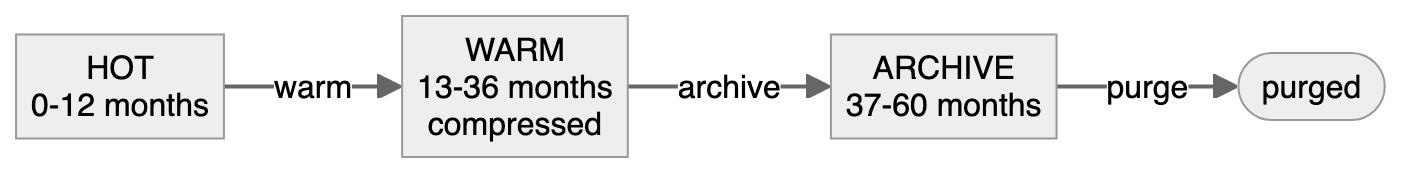
\includegraphics[width=0.62\linewidth]{02_tiers_cover}
  \vfill
  \begin{tabular}{rl}
    \textbf{Team} & \TeamMemberA \\
                  & \TeamMemberB \\[6pt]
    \textbf{Supervisor} & \Supervisor \\[6pt]
    \textbf{Academic year} & \AcademicYear \\[6pt]
    \textbf{Repository} & \small\url{\RepoURL}
  \end{tabular}
\end{titlepage}

\pagenumbering{roman}
\chapter*{Abstract}
\addcontentsline{toc}{chapter}{Abstract}

A mobile telecom operator keeps six years of billing records in a single Oracle table. Monthly
and audit reports slow down as the table grows, purging old data is a long \code{DELETE} that
produces gigabytes of redo, and the legal retention rules are applied by hand. As two
consultants, we were asked to design and evaluate a data lifecycle strategy that combines
partitioning, indexing, compression and archiving, and to prove its effect with measurements.

We built the solution on Oracle Database 19c Enterprise Edition (in Docker) and compared it
with the client's current design on the same synthetic dataset of 23.76 million billing rows
over 72 months. The optimised design partitions the billing table by month with interval
partitioning. A PL/SQL package (\code{DLM\_PKG}) moves every month through four tiers. Hot
months stay uncompressed and writable. Warm months are compressed and read-only. Archived
months are moved to an archive table by two partition exchanges, without copying a row. Months
past the 60-month legal retention are dropped. Each operation is guarded, logged, resumable
after a crash, and validated against control totals captured when the data was loaded.

Measured results: the month-end revenue report reads 54 times fewer blocks and runs 14 times
faster; an audit query on an archived month is 43 times faster. Archiving one month takes
0.42~s instead of 26~s, and purging one takes 0.02~s instead of 5.1~s. The full monthly job,
including the compression step, is 8.9 times faster and produces 3.8 times less redo.
Retained data uses 44\,\% less storage. All 62 retained months match their control totals.
The solution passes 43 automated functional tests and 25 security checks.

\paragraph{Keywords:} Oracle Database 19c, interval partitioning, partition exchange, data
lifecycle management, archiving, basic table compression, partition pruning, retention policy,
PL/SQL, performance benchmarking.

\tableofcontents
\listoffigures
\listoftables
\clearpage
\pagenumbering{arabic}

\chapter{General Introduction}

\section{Context}

Billing is one of the largest data sets of a telecom operator. Each call, SMS, data session
and roaming event becomes a billed line, and those lines must be kept for years for customer
care, finance, disputes and legal audits. In many companies this history accumulates in the
same table that the billing application writes to every day. The table grows without limit,
and work that was cheap when it held one year of data becomes slow with six.

This project was carried out within the \Course{} course. Its brief (Project 22) asks for a
data lifecycle strategy that combines partitioning where it is licensed, indexing, archiving
and performance benchmarking, and for proof of its effect on comparable workloads.

\section{Motivation}

Three symptoms of the client's current design drive the work:

\begin{itemize}
  \item \textbf{Reports slow down every month.} A report on last month's revenue reads the
        whole six-year table, because one month is too large a share of the rows for an
        index to help.
  \item \textbf{Retention is expensive.} Removing a month means \code{DELETE}-ing hundreds of
        thousands of rows. Every row and every index entry generates undo and redo, and the
        table does not even shrink afterwards.
  \item \textbf{Retention is manual and risky.} Nothing prevents someone from deleting data
        that is still under legal retention, and nothing proves afterwards that no billing
        record was lost or changed.
\end{itemize}

\section{Problem statement}

\emph{How can the billing history be organised so that frequent reports read only the period
they need, old data moves to cheaper storage and is removed at the end of its retention with
near-zero cost, while guaranteeing, and proving, that no billing record is lost or altered?}

\section{Objectives}

\begin{enumerate}
  \item Generate a representative, reproducible billing history (tens of millions of rows).
  \item Measure the performance of the current design on a defined workload: the
        \emph{baseline}.
  \item Design a partitioned schema and a lifecycle policy (hot, warm, archive, purge) suited
        to the client's retention rules and licences.
  \item Implement the lifecycle as automated, guarded, logged and recoverable database code.
  \item Measure query, maintenance and storage effects on the same workload, and verify data
        integrity objectively.
  \item Document the licensing restrictions, trade-offs and limits of the solution.
\end{enumerate}

\section{Structure of the report}

Chapter~\ref{ch:client} presents the client. Chapters~\ref{ch:requirements}
and~\ref{ch:technology} analyse the requirements and compare the possible technologies.
Chapter~\ref{ch:architecture} describes the architecture, and
Chapters~\ref{ch:environment} and~\ref{ch:implementation} the environment and the
implementation. Chapter~\ref{ch:usage} shows practical scenarios. Chapters~\ref{ch:testing}
and~\ref{ch:performance} present the tests and the measured results.
Chapters~\ref{ch:challenges} to~\ref{ch:conclusion} discuss the difficulties, the limits and
the outcome. All the code, test outputs and benchmark data are in the project repository
(\url{\RepoURL}).

\chapter{Client Company Presentation}\label{ch:client}

\section{Business sector and company}

The client is a mobile telecom operator (a fictitious company created for this scenario)
serving about 500\,000 subscribers in twelve regions. It sells prepaid, postpaid and business
plans (twenty tariff plans) and bills four kinds of service: voice, SMS, mobile data and
roaming. About 10\,\% of the customers are businesses.

\section{IT environment}

Billing is handled by an in-house application that writes billing lines into an Oracle
database. Finance, customer care, collections and the legal department query the same data.
The database team runs Oracle Database 19c Enterprise Edition, which already includes the
Partitioning option in the client's licence. For this assignment, the database is a 19c
container (Oracle 19.19, ARM64) running under Docker on a team member's laptop, with a single
pluggable database \code{ORCLPDB1}.

\section{Project sponsor}

The project is sponsored by the \textbf{DBA Manager}. They are responsible for the
performance of the billing database, the night maintenance window, and compliance with the
retention rules defined by the legal department.

\section{Business requirements}

\begin{itemize}
  \item Month-end finance reports and customer-care screens must stay fast even as history
        grows.
  \item Billing data must be kept for \textbf{60 months} (legal retention) and then deleted.
  \item Data older than three years is rarely read but must stay queryable for audits and
        disputes.
  \item The billing application must never be blocked, and must never be able to change or
        delete history.
  \item Every retention action must be traceable and provably safe.
\end{itemize}

\section{Operational constraints}

\begin{table}[H]
\centering
\caption{Operational constraints}
\begin{tabularx}{\linewidth}{lL}
\toprule
Constraint & Description \\
\midrule
Availability & Lifecycle operations must not stop the billing application (partition-level work, short locks). \\
Security & Least privilege, no credentials in code, read-only history, audit trail. \\
Performance & Reports filtered on dates must read only the requested period. \\
Licensing & Use only features covered by Enterprise Edition + Partitioning; no Advanced Compression, no Diagnostics/Tuning Packs. \\
Resources & Laptop with Docker: 8 vCPU and about 8~GB of RAM for Docker; the disk was nearly full (about 20~GB free at the start). \\
Schedule & Four weeks: design, implementation, tests and measurements, deliverables. \\
Data & Synthetic, anonymised data only. \\
\bottomrule
\end{tabularx}
\end{table}

\chapter{Requirements Analysis and Project Specifications}\label{ch:requirements}

\section{Functional requirements}

\begin{table}[H]
\centering
\caption{Functional requirements}
\begin{tabularx}{\linewidth}{lL}
\toprule
ID & Requirement \\
\midrule
F1 & Store the billing history so that monthly and annual reports read only the period requested. \\
F2 & Apply the retention policy automatically: hot (12 months), online (36 months), archive (until 60 months), purge after. \\
F3 & Keep archived data queryable (audit, legal requests) through a single access point. \\
F4 & Allow the retention parameters to change without modifying code. \\
F5 & Provide a dry-run mode that shows what the job would do. \\
F6 & Log every lifecycle action: what, when, how many rows, how long, result. \\
F7 & Prove the integrity of billing data after every operation. \\
\bottomrule
\end{tabularx}
\end{table}

\section{Technical and non-functional requirements}

\begin{table}[H]
\centering
\caption{Technical requirements}
\begin{tabularx}{\linewidth}{lL}
\toprule
ID & Requirement \\
\midrule
T1 & Lifecycle operations must avoid copying or deleting rows one by one where possible. \\
T2 & A failure in the middle of an operation must not lose data, and a re-run must recover. \\
T3 & Data inside the legal retention can never be purged, whatever parameter is passed. \\
T4 & Old billing data cannot be modified (by accidental updates or late inserts). \\
T5 & Least privilege: the billing application cannot delete history or run lifecycle jobs, and analysts are read-only. \\
T6 & No credentials in source code or in the Git repository. \\
T7 & The whole solution must be reproducible from scripts on the course Docker environment. \\
T8 & The lab must not exhaust the laptop disk. \\
T9 & Use only licensed features, and document the licence impact. \\
\bottomrule
\end{tabularx}
\end{table}

\section{Retention policy}

The legal and business rules translate into four tiers, stored as parameters in the
\code{DLM\_CONFIG} table rather than hard-coded:

\begin{table}[H]
\centering
\caption{Retention policy parameters}
\begin{tabularx}{\linewidth}{llL}
\toprule
Parameter & Value & Meaning \\
\midrule
\code{HOT\_MONTHS} & 12 & months kept uncompressed and writable \\
\code{ONLINE\_MONTHS} & 36 & months kept in the online billing table (hot + warm) \\
\code{RETENTION\_MONTHS} & 60 & legal retention; older months are purged \\
\code{MIN\_RETENTION\_MONTHS} & 60 & safety floor: no purge may use a shorter retention \\
\code{AS\_OF\_MONTH} & 2026-11 & reference ``today'', so that runs are reproducible \\
\bottomrule
\end{tabularx}
\end{table}

\section{Measurable indicators and acceptance criteria}

We formalised the indicators after a first exploratory benchmark and before the final run
whose numbers this report presents. The brief asks for indicators to be defined before
testing, so we state this order openly. The indicators compare the two designs on the same
data, with the same SQL text and bind values.

\begin{table}[H]
\centering
\caption{Key performance indicators and targets}
\label{tab:kpi}
\begin{tabularx}{\linewidth}{lXl}
\toprule
KPI & Indicator & Target \\
\midrule
K1 & Month-end report (Q1): elapsed time and logical reads & $\geq$5$\times$ time, $\geq$10$\times$ LIO \\
K2 & Audit query on an archived month (Q7) & $\geq$5$\times$ fewer LIO \\
K3 & OLTP lookups (Q2 by customer, Q5 by id) & no time regression $>$2$\times$ \\
K4 & Archive one month (and the whole monthly job) & $\geq$10$\times$ faster, $<$5~s \\
K5 & Purge one month & $<$1~s \\
K6 & Monthly load + statistics refresh & not slower than baseline \\
K7 & Storage of the retained data & $\geq$25\,\% smaller \\
K8 & Data integrity vs load-time control totals & 100\,\% of months \\
K9 & Recovery after a crash & 0 rows lost, recovery = re-run \\
K10 & Security controls (asserted checks) & 100\,\% \\
K11 & Automation & one command per month \\
\bottomrule
\end{tabularx}
\end{table}

The acceptance criteria of the brief are: (1) the design preserves data integrity,
(2) retention operations work correctly, (3) query or maintenance improvements are measured
on comparable workloads, and (4) licensing restrictions and technical trade-offs are
documented. Chapter~\ref{ch:performance} checks each of them.

\chapter{Technology Assessment and Justification}\label{ch:technology}

\section{Database platform}

The brief allows Oracle Database Free \emph{if supported by the selected version} or a
licensed 19c when required. We checked the course container before choosing:
\code{V\$OPTION} reports \code{Partitioning = TRUE}, and a test interval-partitioned table
could be created and dropped.

\begin{table}[H]
\centering
\caption{Database platform options}
\begin{tabularx}{\linewidth}{>{\raggedright\arraybackslash}p{3.4cm}LL>{\raggedright\arraybackslash}p{2.1cm}}
\toprule
Option & Advantages & Drawbacks & Decision \\
\midrule
Oracle Database 23ai Free & free, recent, partitioning available & 12~GB user data, 2~GB RAM, not the course environment & not needed \\
Oracle 19c EE (course container) & installed, Partitioning option present, long-term support release used by most companies & EE and Partitioning are paid options in production & \textbf{chosen} \\
\bottomrule
\end{tabularx}
\end{table}

\section{Data segmentation}

\begin{table}[H]
\centering
\caption{Segmentation options}
\begin{tabularx}{\linewidth}{>{\raggedright\arraybackslash}p{3.4cm}LL>{\raggedright\arraybackslash}p{2.1cm}}
\toprule
Option & Advantages & Drawbacks & Decision \\
\midrule
Single heap table + indexes (current) & simple & full scans for period reports; retention by \code{DELETE} & baseline \\
One table per month + \code{UNION ALL} view & works without the Partitioning option & views to regenerate monthly, inserts must be routed, weaker pruning with binds & documented alternative \\
Range partitioning with a job creating partitions & standard & inserts fail if the job is late & rejected \\
\textbf{Interval-range partitioning by month on \code{bill\_date}} & partitions created automatically, pruning, partition-level maintenance & Partitioning option, system-generated names & \textbf{chosen} \\
Composite range-list (by service) & finer pruning on service & more segments; the workload does not filter on service alone & rejected \\
\bottomrule
\end{tabularx}
\end{table}

A \textbf{month} is the right partition unit because the retention rule, the billing cycle
and most reports are monthly. One month holds about 230\,000 to 430\,000 rows (20--35~MB),
so each partition can be scanned, moved, exchanged or dropped in seconds.

\section{Archiving method}

\begin{table}[H]
\centering
\caption{Archiving options}
\begin{tabularx}{\linewidth}{>{\raggedright\arraybackslash}p{3.4cm}LL>{\raggedright\arraybackslash}p{2.1cm}}
\toprule
Option & Advantages & Drawbacks & Decision \\
\midrule
\code{INSERT ... SELECT} + \code{DELETE} (current) & simple & copies and deletes every row; large redo and undo; table does not shrink & baseline \\
Data Pump export of old partitions + drop & data leaves the database & no longer queryable in SQL; restore needed for audits & rejected (F3) \\
\textbf{Exchange partition into an archive table} & metadata operation; archive stays queryable & global index maintenance; identical structures required & \textbf{chosen} \\
\bottomrule
\end{tabularx}
\end{table}

\section{Compression and licensing}

\begin{table}[H]
\centering
\caption{Compression options}
\begin{tabularx}{\linewidth}{>{\raggedright\arraybackslash}p{4.2cm}L>{\raggedright\arraybackslash}p{3.6cm}}
\toprule
Option & Licence & Decision \\
\midrule
\textbf{BASIC} (\code{ROW STORE COMPRESS BASIC}) & included in Enterprise Edition (not available in SE2) & \textbf{chosen} for read-only data \\
ADVANCED (OLTP) & Advanced Compression option & not used (licence) \\
Hybrid Columnar Compression & Exadata or engineered storage only & not available \\
\bottomrule
\end{tabularx}
\end{table}

BASIC compression only compresses direct-path operations, and conventional updates on
compressed blocks are inefficient. That fits warm and archived data, which is written once by
\code{MOVE PARTITION} and then made read-only. The measurement method relies only on
base-product views (\code{V\$MYSTAT}, \code{V\$SQL}, \code{DBMS\_XPLAN.DISPLAY\_CURSOR}).
We deliberately did not use AWR, ASH or SQL Monitor, which need the Diagnostics and Tuning
Packs.

\section{Tooling}

\begin{table}[H]
\centering
\caption{Tooling choices}
\begin{tabularx}{\linewidth}{>{\raggedright\arraybackslash}p{3cm}>{\raggedright\arraybackslash}p{4.6cm}L}
\toprule
Need & Choice & Reason \\
\midrule
Lifecycle logic & PL/SQL package & runs next to the data, transactional logging, schedulable \\
Data generation & set-based SQL with \code{ORA\_HASH} & millions of rows per minute, deterministic \\
Benchmark harness & Python 3.12 + python-oracledb & session statistics, plans, JSON, charts \\
SQL clients & SQL*Plus (DB container), SQLcl (tools) & nothing installed on the host \\
Automation & Bash scripts + Docker Compose & reproducible on any Docker host \\
Demonstration interface & Streamlit web dashboard (tools image) & every scenario by clicks, no terminal; calls the same package \\
Version control & Git, GitHub & required by the brief \\
\bottomrule
\end{tabularx}
\end{table}

\chapter{System Design and Architecture}\label{ch:architecture}

\section{Overall architecture}

Figure~\ref{fig:architecture} shows the components and their interactions. Three kinds of
clients use the database, each through a different account and access path:

\begin{itemize}
  \item The \textbf{billing application} (\code{TELCO\_APP}) writes and reads through the view
        \code{BILLING\_CURRENT\_V}. The view exposes only the hot months and rejects any row
        outside them.
  \item \textbf{Analysts and auditors} (\code{TELCO\_ANALYST}) read the whole retained history
        through \code{BILLING\_ALL}, the union of the online and archive tables.
  \item The \textbf{DBA or scheduler} (\code{TELCO\_OWNER}) runs the lifecycle package
        \code{DLM\_PKG}. The package reads its policy from \code{DLM\_CONFIG}, logs to
        \code{DLM\_JOB\_LOG} and validates against \code{BILLING\_CONTROL\_TOTALS}.
\end{itemize}

The benchmark harness runs in a separate tools container and reaches the database over TCP.
The baseline tables (\code{BILLING\_RECORDS\_BASE}, \code{BILLING\_ARCHIVE\_BASE}) live in the
same schema, so both designs are compared on the same server, data and workload.

\begin{sidewaysfigure}
  \centering
  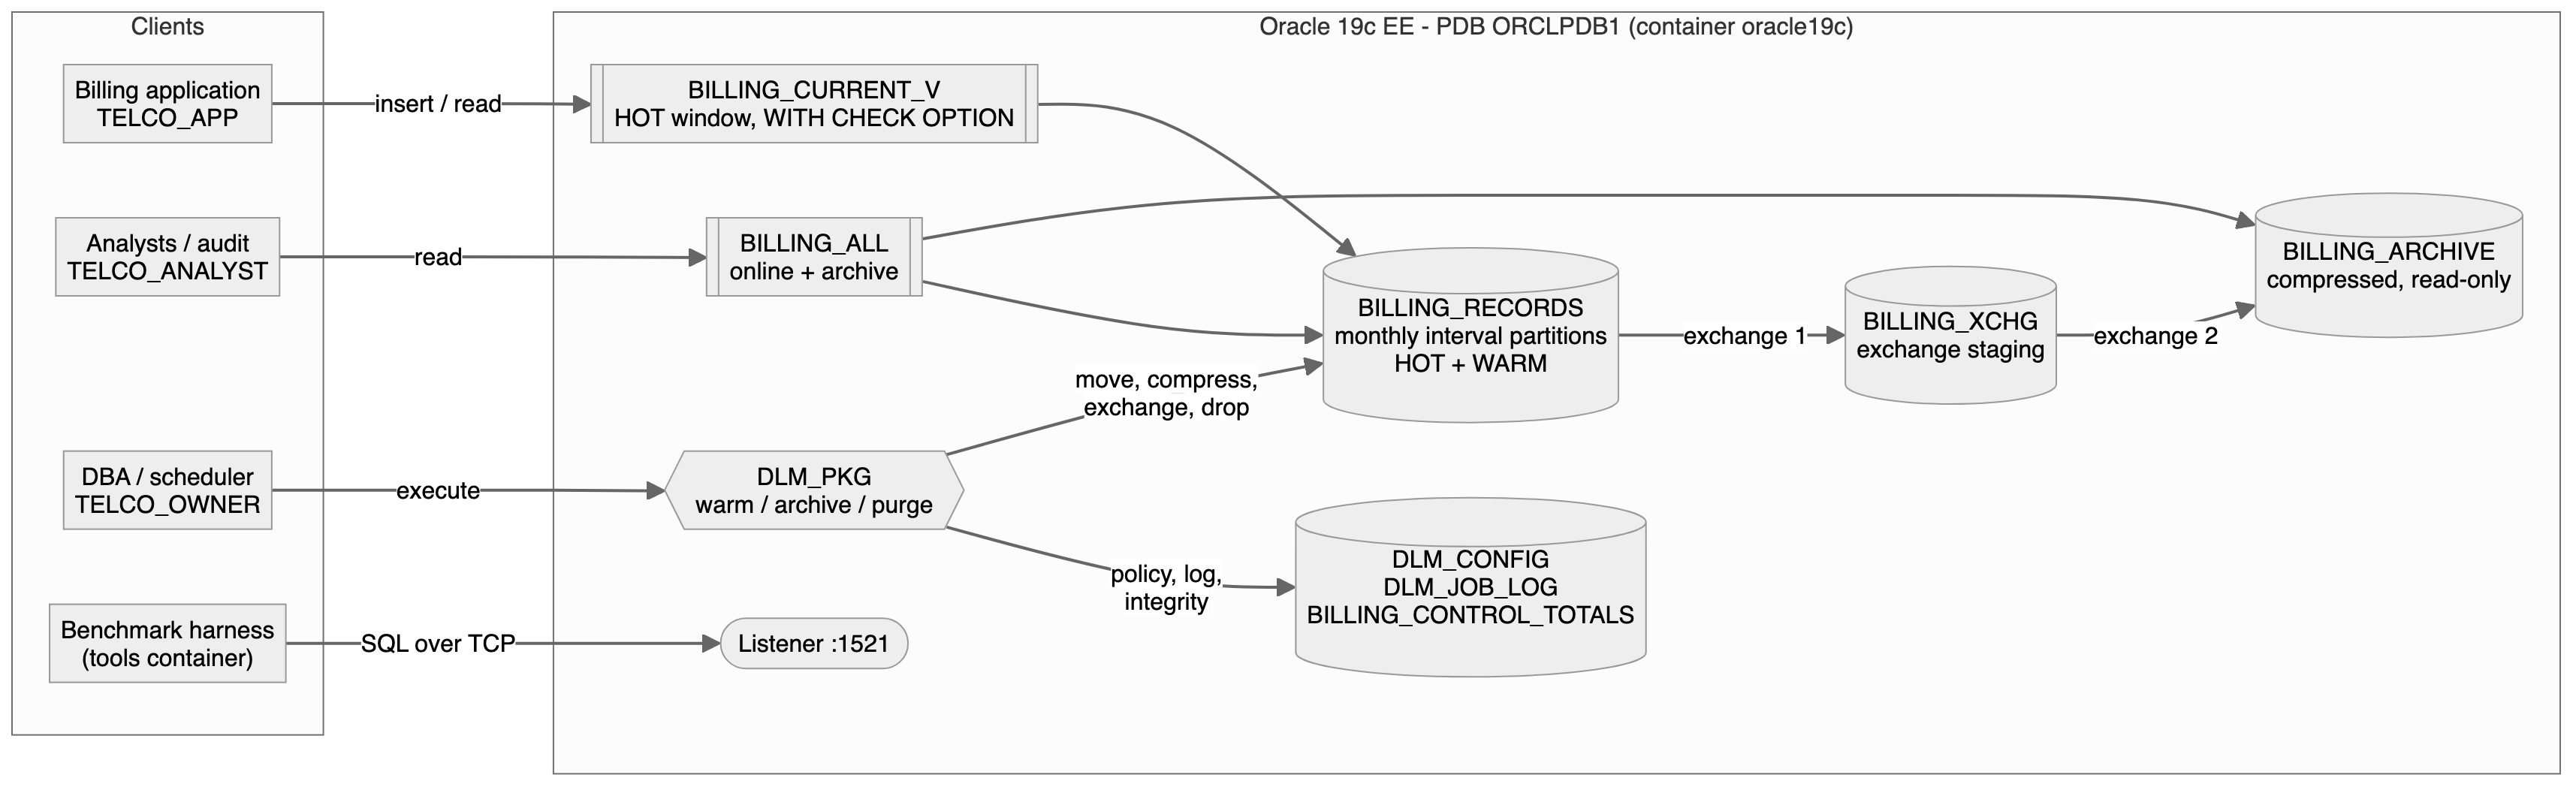
\includegraphics[width=\linewidth]{01_architecture}
  \caption{Overall system architecture}
  \label{fig:architecture}
\end{sidewaysfigure}

\section{Storage tiers and data lifecycle}

Each month moves through four states (Figure~\ref{fig:tiers}). Each state has its own
tablespace, storage format and access rights. Tablespaces separate the tiers physically:
\code{TELCO\_HOT} for current data, \code{TELCO\_IDX} for its indexes, and \code{TELCO\_ARCH}
for compressed warm and archived data. In production, \code{TELCO\_ARCH} could sit on cheaper
storage.

\begin{figure}[H]
  \centering
  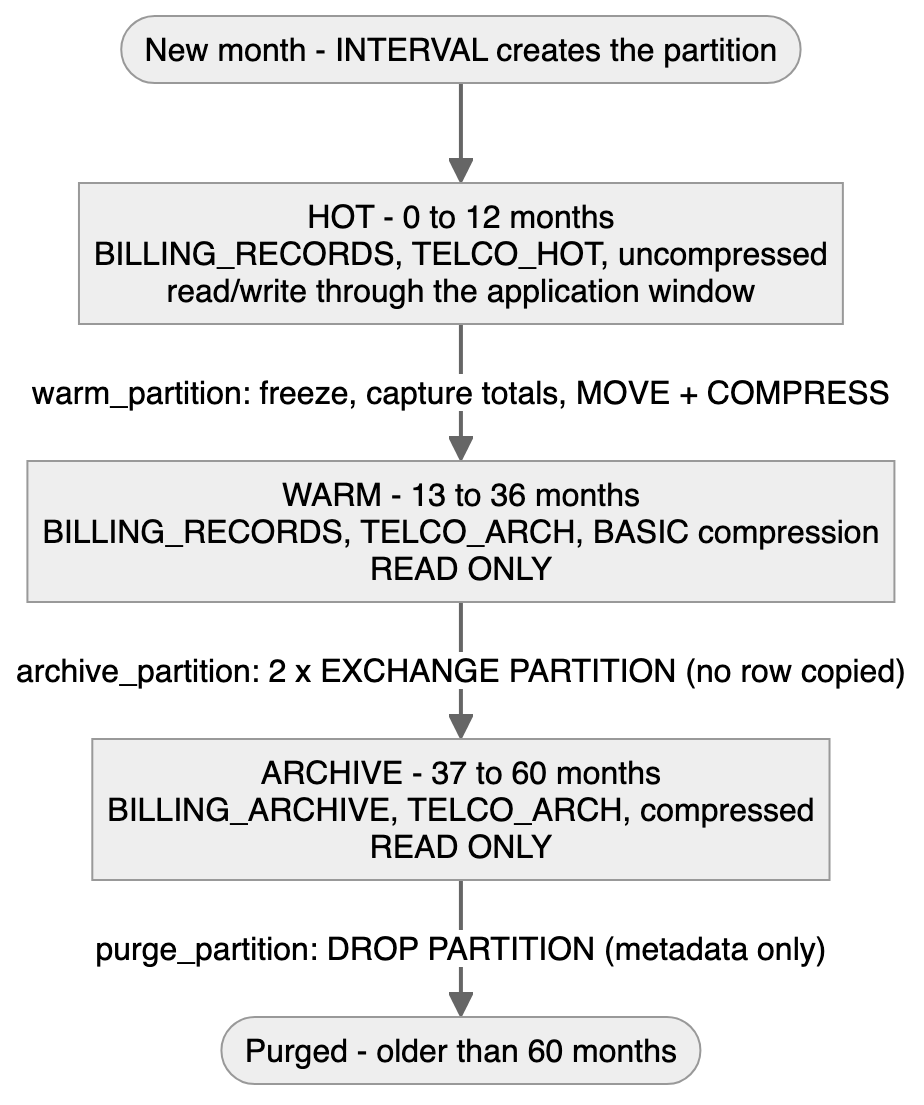
\includegraphics[width=0.62\linewidth]{02_tiers}
  \caption{Storage tiers and lifecycle operations}
  \label{fig:tiers}
\end{figure}

\begin{description}[style=nextline]
  \item[HOT (0--12 months)] Uncompressed in \code{TELCO\_HOT}. The application may insert
        late lines and corrections here through its window view.
  \item[WARM (13--36 months)] The month is \emph{frozen}: it is set read-only, its control
        totals are re-captured, and it is moved to \code{TELCO\_ARCH} with BASIC compression.
        It stays in \code{BILLING\_RECORDS}, so recent-history queries use the same table.
  \item[ARCHIVE (37--60 months)] The month leaves the online table for
        \code{BILLING\_ARCHIVE} through two partition exchanges, and stays compressed and
        read-only.
  \item[PURGED ($>$60 months)] The archive partition is dropped, which is a metadata operation.
\end{description}

\section{Archive sequence}

The key mechanism is the zero-copy archive (Figure~\ref{fig:sequence}). A partition can only
be exchanged with a non-partitioned table, so the month travels through the empty staging
table \code{BILLING\_XCHG}. Step~1 swaps the month's segment into the staging table. Step~2
creates the archive partition (\code{LOCK TABLE ... PARTITION FOR}) and swaps the segment into
it. Step~3 drops the now-empty online partition. No row is copied at any point. If the job
dies between steps 1 and 2, the data waits in \code{BILLING\_XCHG}: the integrity check
reports the month as missing, and the next run detects the staged rows and resumes at step~2.

\begin{sidewaysfigure}
  \centering
  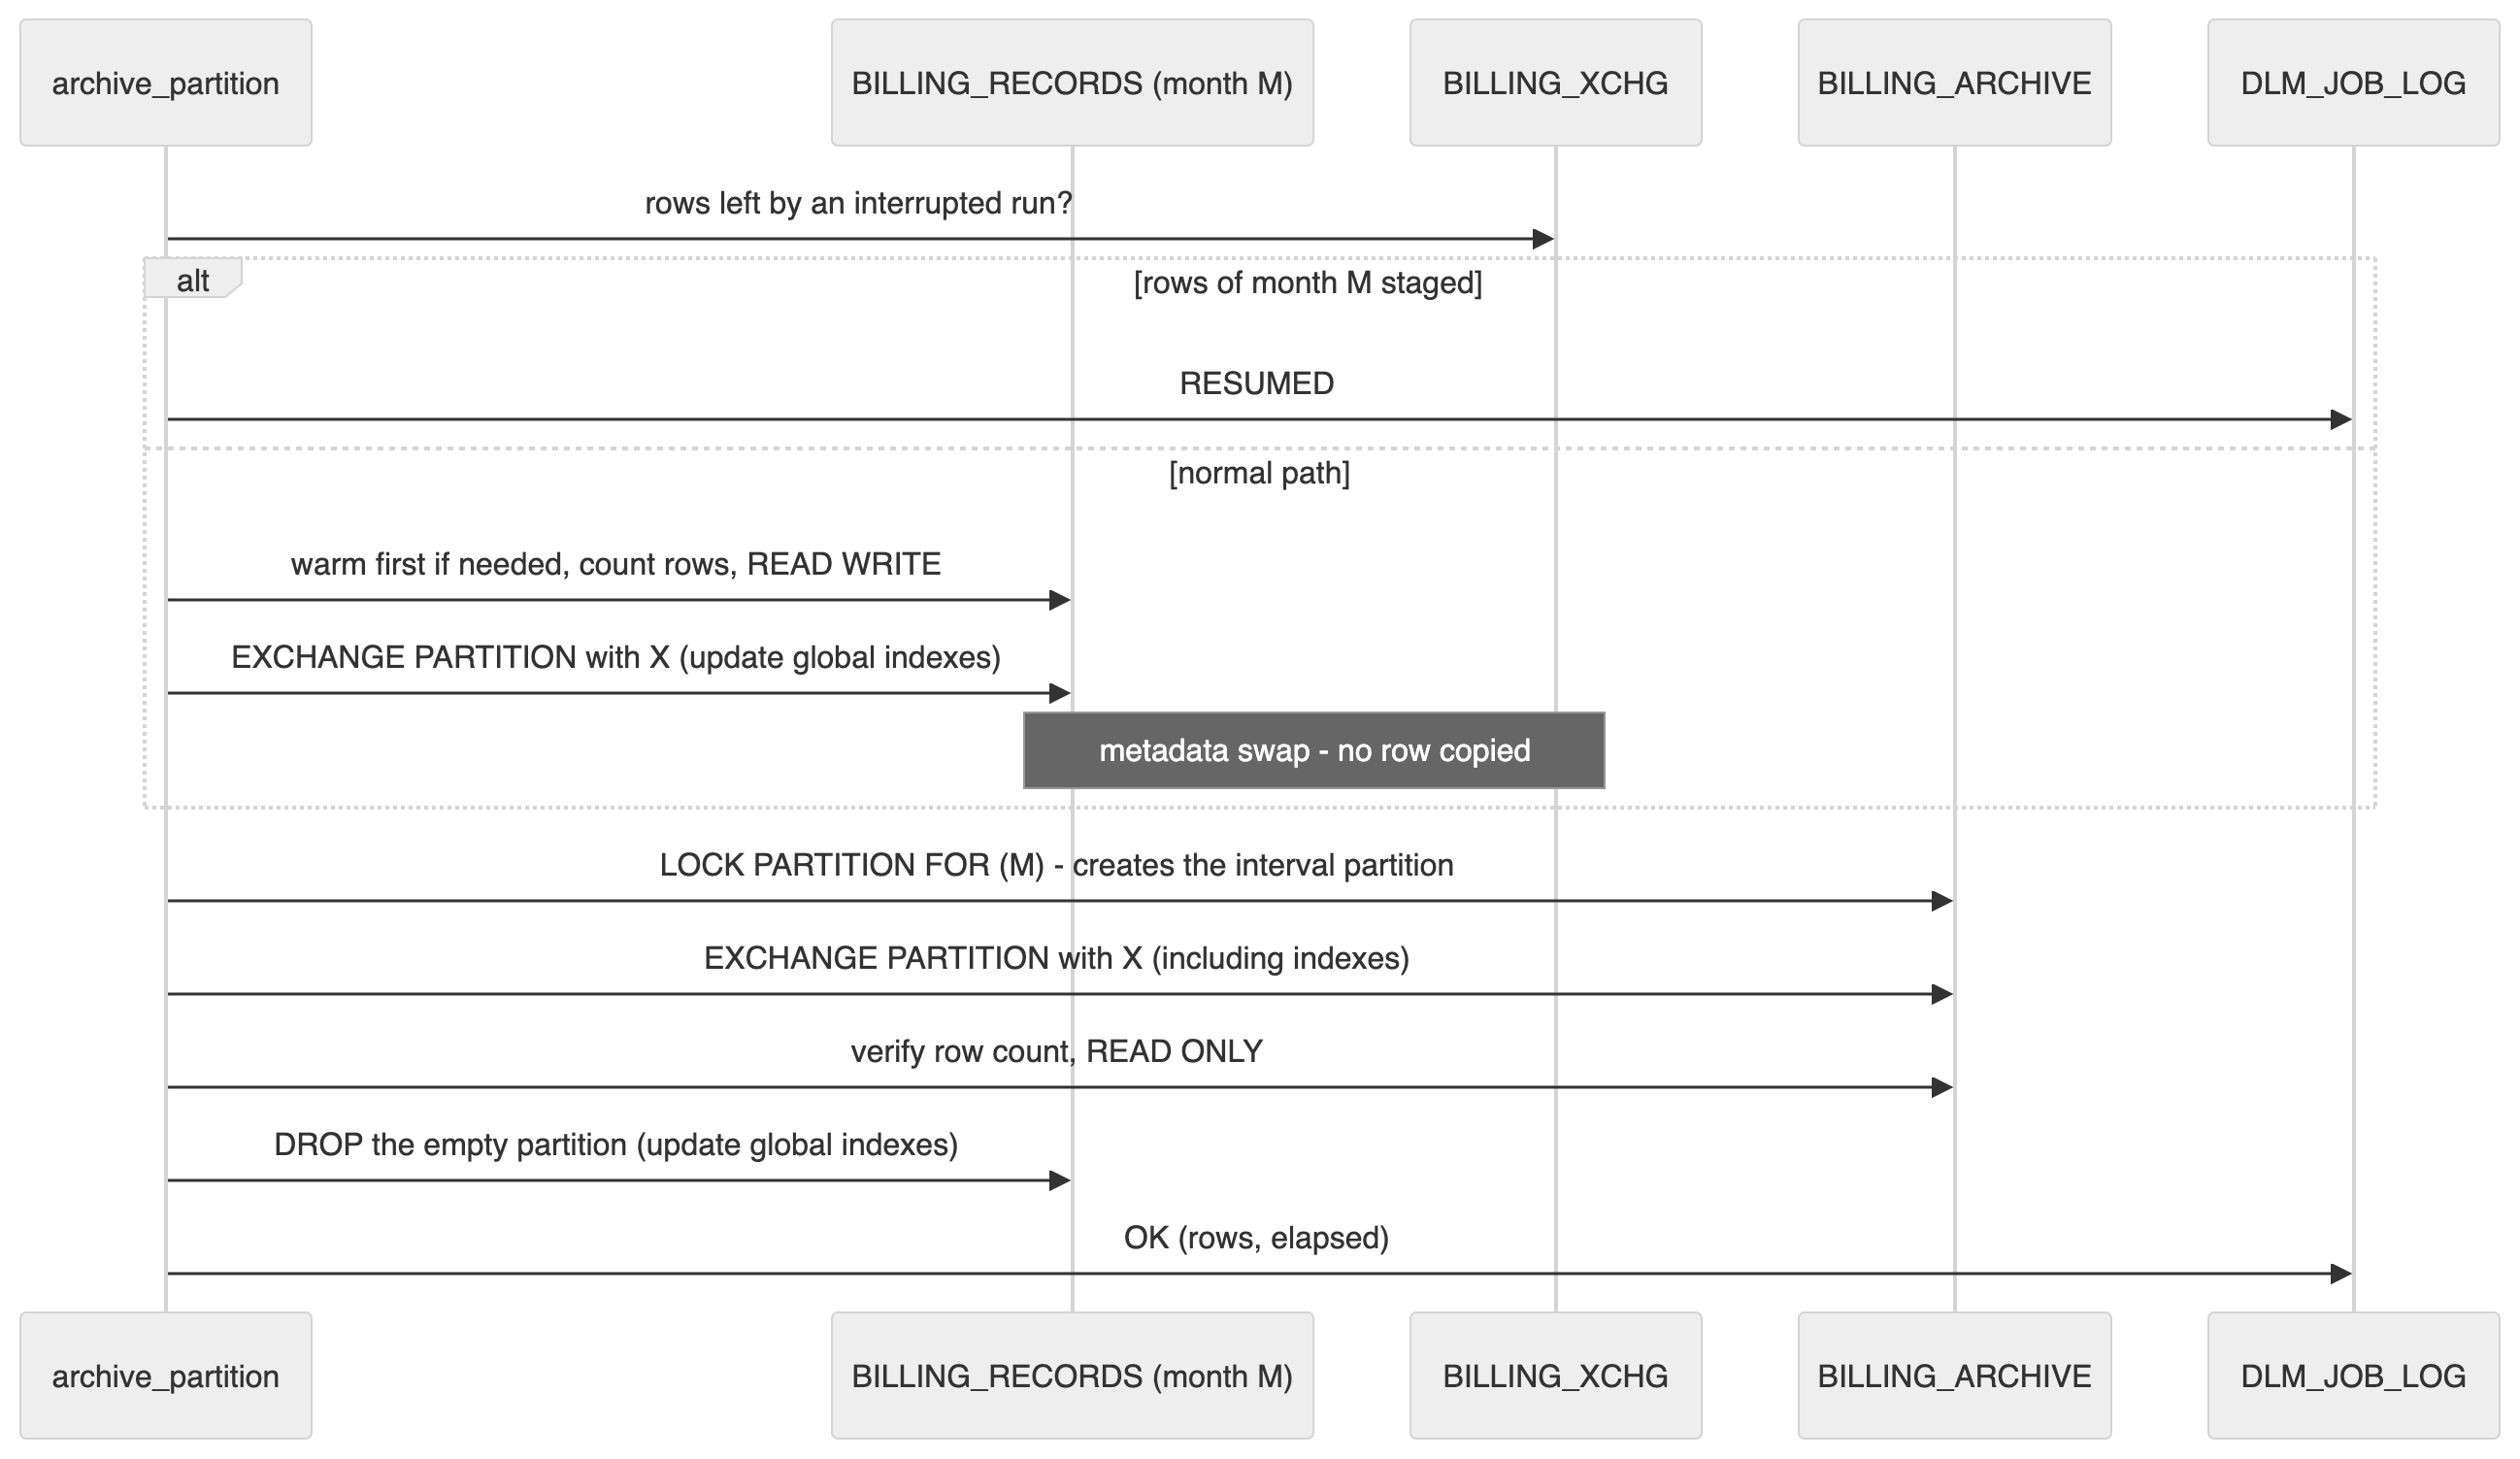
\includegraphics[width=0.95\linewidth]{03_archive_sequence}
  \caption{Archive of one month: sequence diagram}
  \label{fig:sequence}
\end{sidewaysfigure}

\section{Monthly job (activity)}

\code{run\_lifecycle} orchestrates a complete monthly run (Figure~\ref{fig:activity}). It
first closes the application window on the months it is about to freeze, then resumes any
interrupted archive, removes empty partitions left by rejected inserts, and re-applies
read-only on archive partitions. It then purges, warms and archives, refreshes incremental
statistics and validates every frozen month. If a frozen month differs from its control
totals, the job stops with \code{ORA-20040} so that an operator investigates.

\begin{figure}[H]
  \centering
  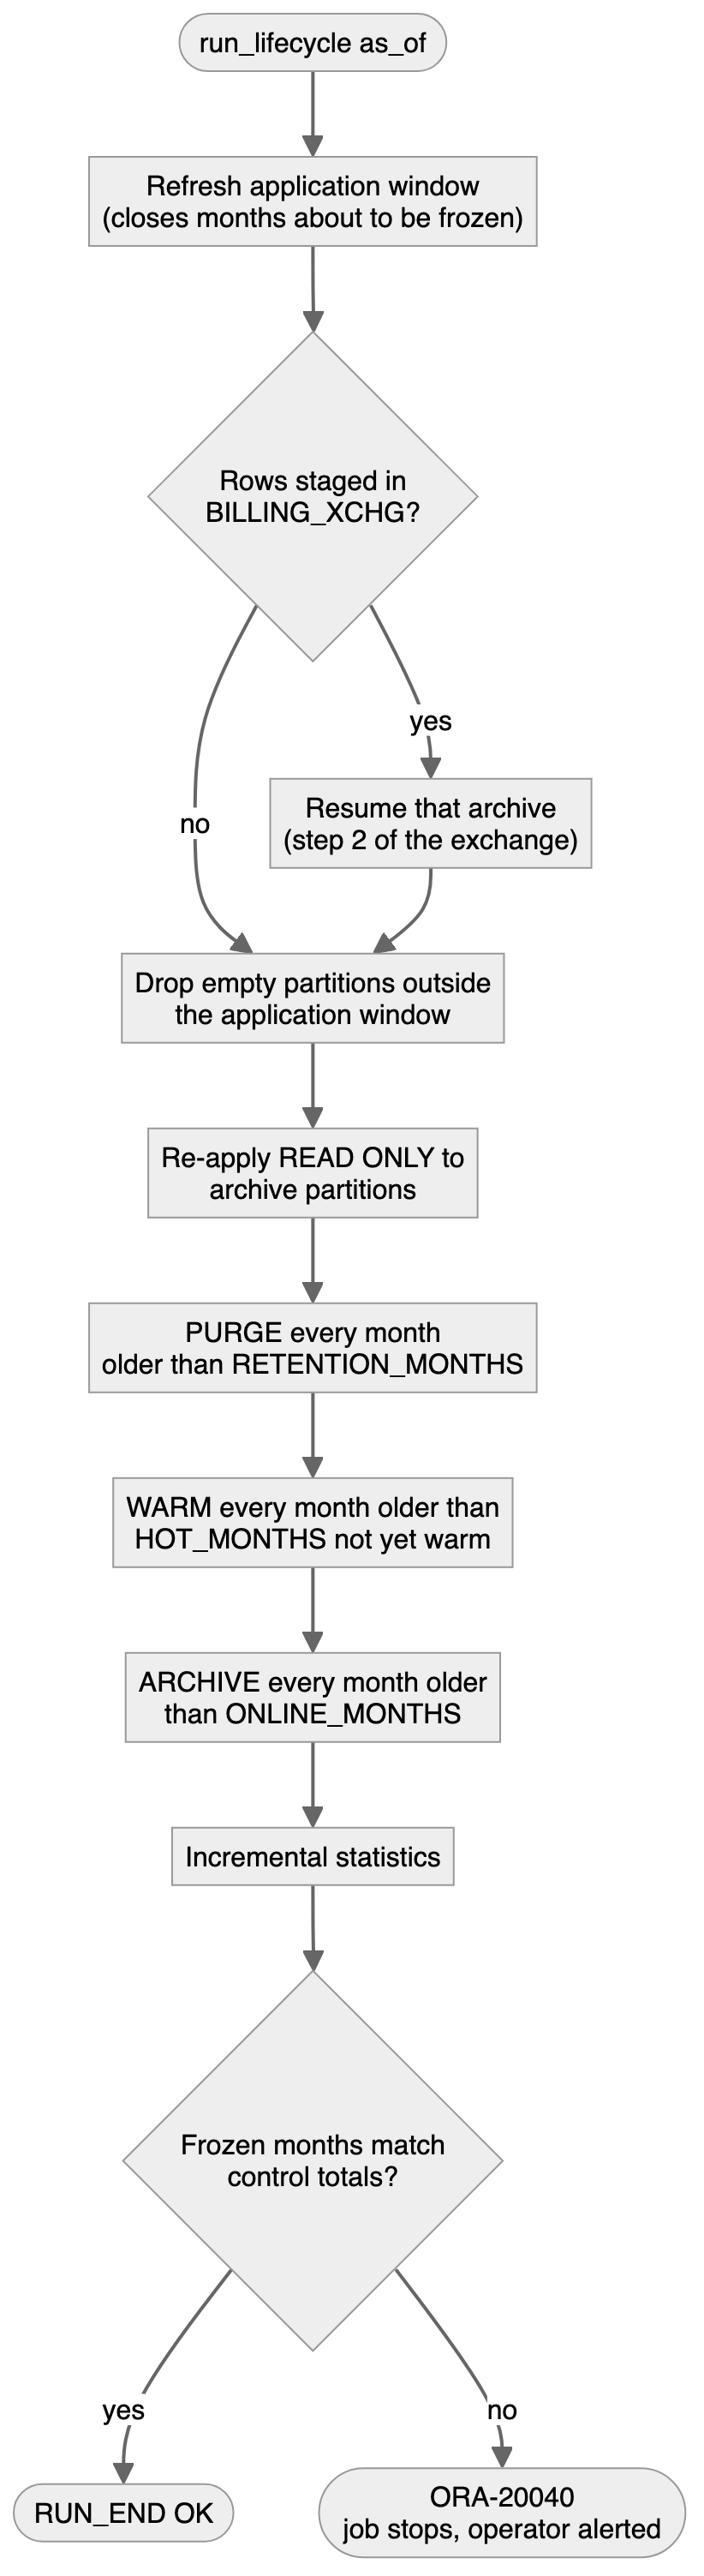
\includegraphics[height=0.72\textheight]{05_lifecycle_activity}
  \caption{Monthly lifecycle job: activity diagram}
  \label{fig:activity}
\end{figure}

\section{Logical data model}

\begin{figure}[H]
  \centering
  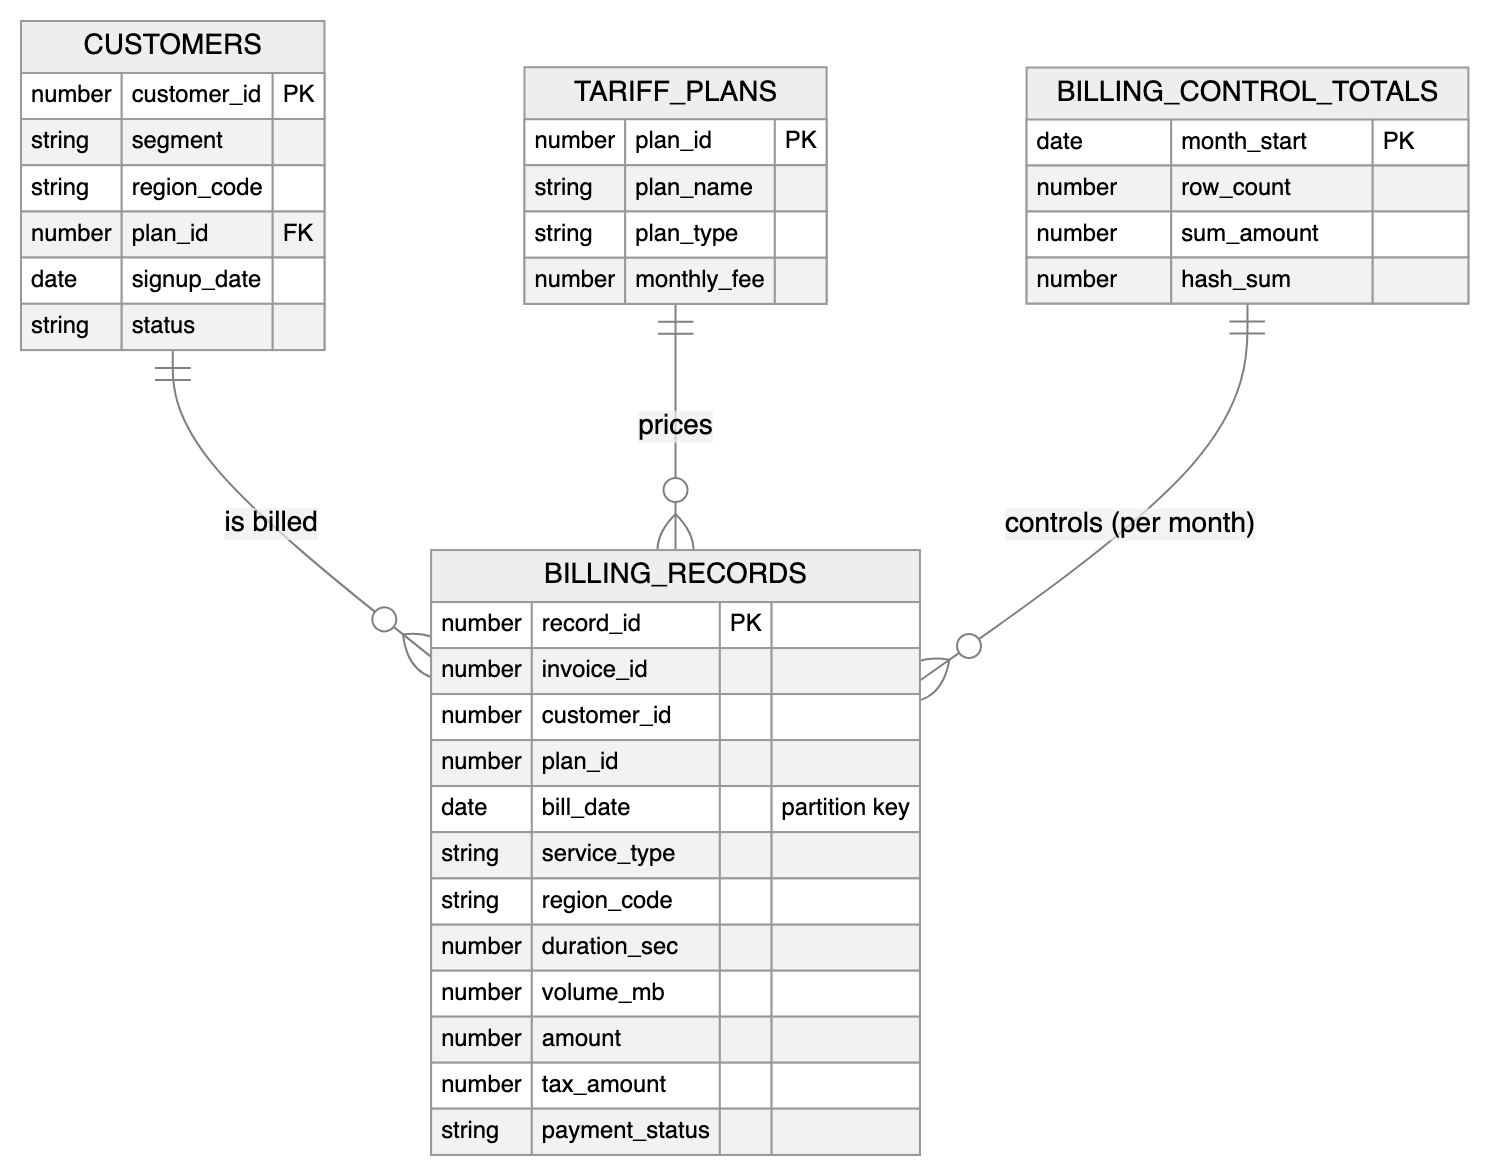
\includegraphics[width=0.85\linewidth]{04_data_model}
  \caption{Logical data model}
  \label{fig:datamodel}
\end{figure}

\code{BILLING\_RECORDS} is the fact table (one row per billed service line). Each customer
subscribes to one tariff plan (\code{CUSTOMERS.plan\_id}, foreign key), and the plan is copied
on every billing line. The other billing
tables (\code{BILLING\_ARCHIVE}, \code{BILLING\_XCHG}, the baseline tables and the load
staging table) are created from \code{BILLING\_RECORDS\_BASE} with
\code{CREATE TABLE ... AS SELECT ... WHERE 1=0}. This guarantees identical columns, which
partition exchange requires. The same \code{CHECK} constraints (service type, payment status,
non-negative amounts) are added to every billing table. There is no foreign key from the fact
table to \code{CUSTOMERS}: as in most billing and warehouse designs, the loading process
guarantees referential integrity, and a foreign key would complicate exchanges and slow bulk
loads.

\section{Indexing strategy}

\begin{table}[H]
\centering
\caption{Indexes of both designs}
\begin{tabularx}{\linewidth}{lllL}
\toprule
Design & Columns & Type & Purpose \\
\midrule
Baseline & \code{record\_id} & PK, B-tree & OLTP lookup \\
Baseline & \code{(customer\_id, bill\_date)} & B-tree & customer history \\
Baseline & \code{bill\_date} & B-tree & date-range reports \\
Partitioned & \code{record\_id} & PK, \textbf{global} B-tree & single probe for any online month \\
Partitioned & \code{(customer\_id, bill\_date)} & \textbf{local} B-tree & one segment per month, moves with it \\
Partitioned & \emph{none on} \code{bill\_date} & -- & replaced by partition pruning \\
Archive & \code{(customer\_id, bill\_date)} & local B-tree & swapped in by \code{INCLUDING INDEXES} \\
\bottomrule
\end{tabularx}
\end{table}

The main trade-off is the global primary key. It keeps lookups by \code{record\_id} to a single
probe, but it must be maintained (\code{UPDATE GLOBAL INDEXES}) whenever a partition is moved
or exchanged out. A local unique index must contain the partition key (ORA-14039), so the
alternative would be a local primary key on \code{(record\_id, bill\_date)}. Lifecycle
operations would then be pure metadata, but \code{record\_id} alone would no longer be
guaranteed unique, and lookups by \code{record\_id} would probe every partition.

\section{Security architecture}

\begin{table}[H]
\centering
\caption{Accounts and privileges (least privilege)}
\begin{tabularx}{\linewidth}{lLL}
\toprule
Account & Privileges & Cannot \\
\midrule
\code{TELCO\_OWNER} & owns the objects, runs DLM, \code{SELECT} on a few \code{V\$} views for benchmarking & -- (would be locked in production, with the job run by a scheduler) \\
\code{TELCO\_APP} & \code{INSERT}, \code{READ} on \code{BILLING\_CURRENT\_V}; \code{READ} on reference data & write outside the hot window, touch base tables, update or delete, read the archive or the policy, run DLM, DDL \\
\code{TELCO\_ANALYST} & \code{READ} on \code{BILLING\_ALL} and reference data & modify anything, lock tables, access base tables, policy or DLM \\
\bottomrule
\end{tabularx}
\end{table}

The other security measures are:

\begin{itemize}
  \item \textbf{No credentials in code or in Git.} A git-ignored \code{.env} (mode 600) is
        generated with random passwords. Passwords are sent to SQL*Plus through standard
        input, so they never appear in the process list. They are only used in
        \code{CREATE/ALTER USER} statements, which Oracle does not keep in clear text in
        \code{V\$SQL}.
  \item \textbf{\code{READ} instead of \code{SELECT}} for read-only accounts. With
        \code{SELECT}, an account can \code{LOCK TABLE} a view and block the lifecycle job; we
        verified this on the database. \code{READ} prevents it.
  \item \textbf{Frozen data is read-only} (ORA-14466 on any change). The application window
        rejects late rows in old months (ORA-01402).
  \item \textbf{Guards and audit trail.} Purges inside the legal retention are refused, and
        every action, refusal and error is logged.
\end{itemize}

\chapter{Implementation Environment}\label{ch:environment}

\section{Hardware and software}

\begin{sidewaysfigure}
  \centering
  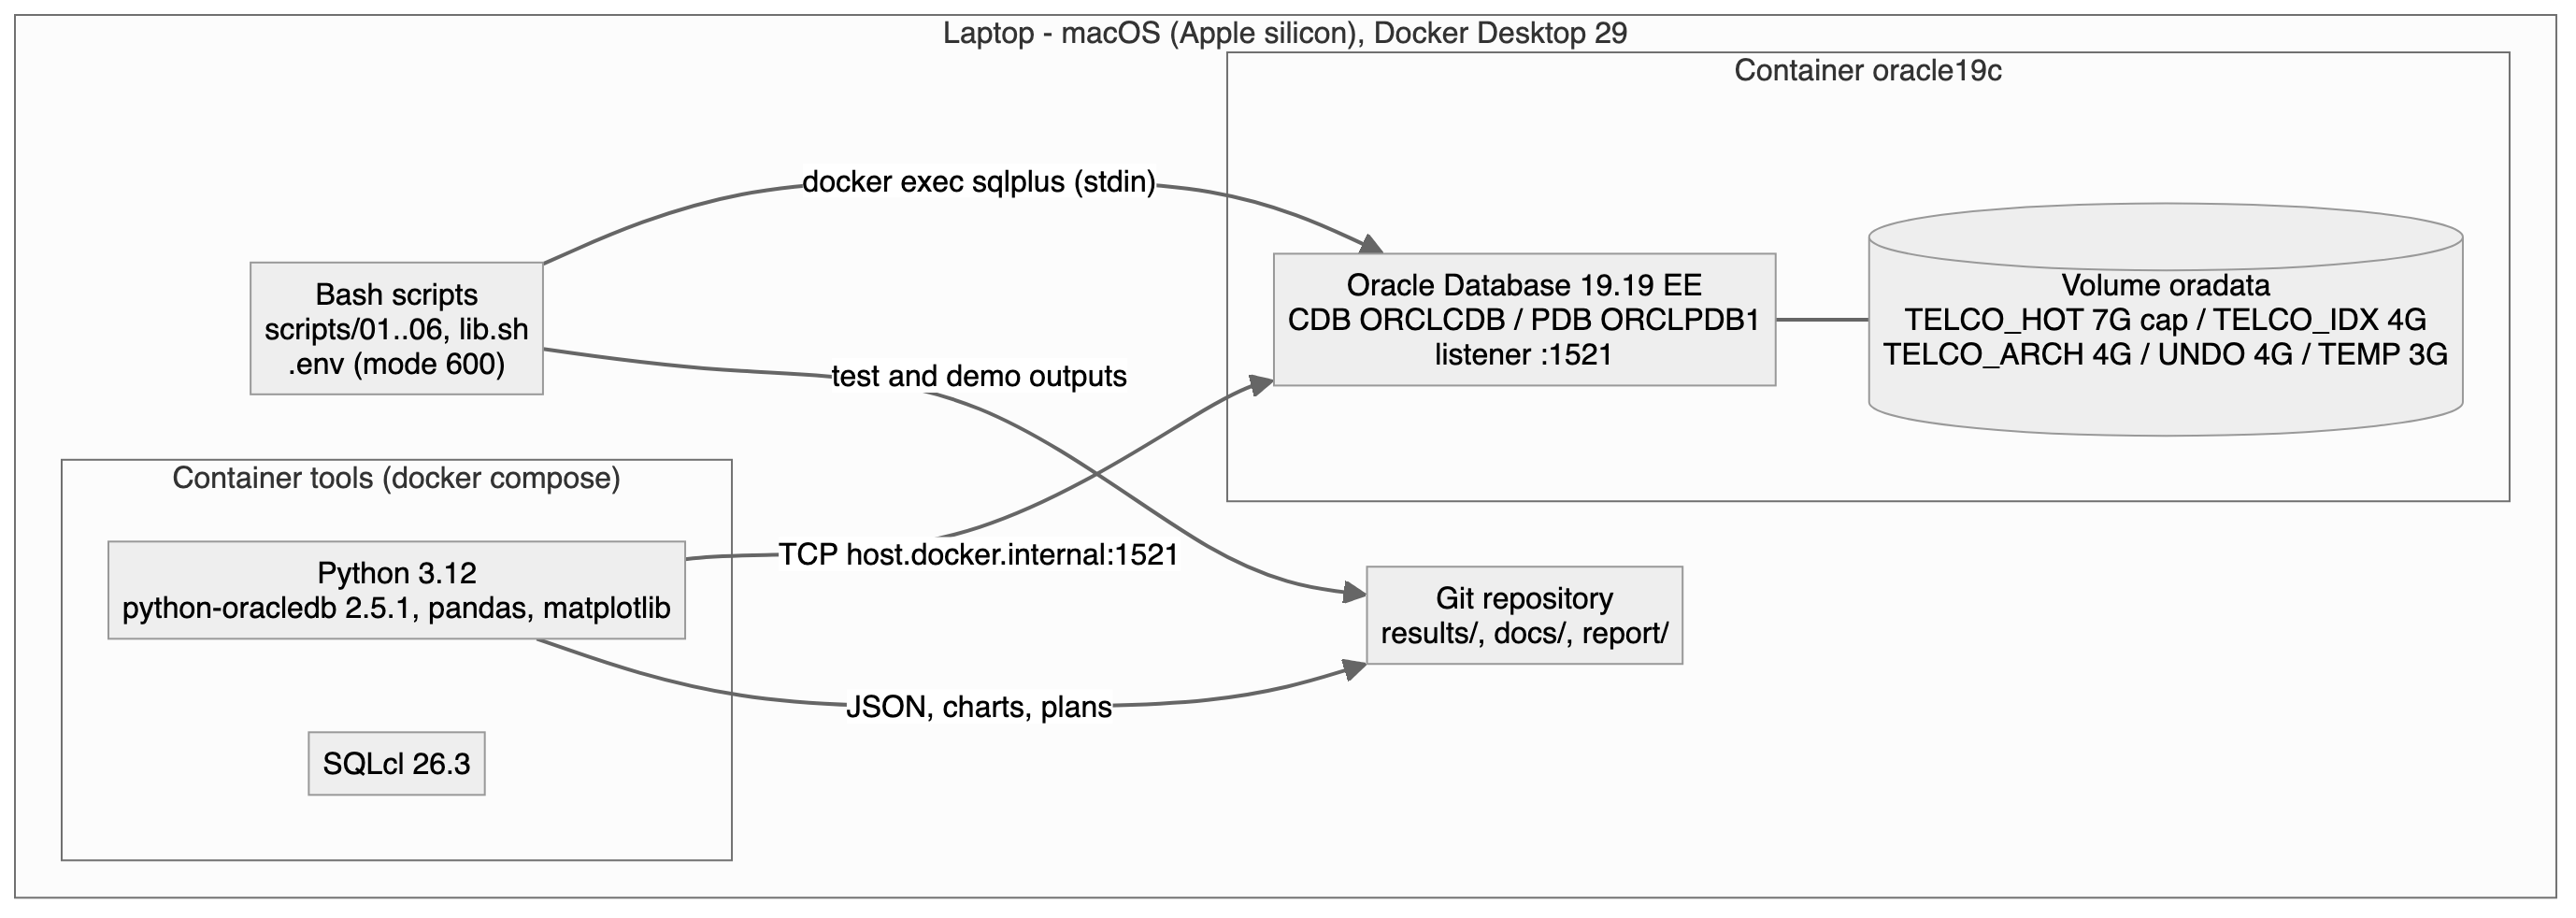
\includegraphics[width=0.9\linewidth]{06_deployment}
  \caption{Deployment diagram}
  \label{fig:deployment}
\end{sidewaysfigure}

Figure~\ref{fig:deployment} shows where each component runs. The database and the tools run in
two containers on the same laptop; the scripts drive SQL*Plus inside the database container
and the benchmark connects over TCP.

\begin{table}[H]
\centering
\caption{Environment and versions}
\begin{tabularx}{\linewidth}{lL}
\toprule
Component & Version / configuration \\
\midrule
Host & Apple silicon laptop, macOS, Docker Desktop 29.0 (8 vCPU, about 8~GB RAM for the Docker VM) \\
Database & Oracle Database 19c Enterprise Edition 19.19 (ARM64), container \code{oracle19c}, CDB \code{ORCLCDB}, PDB \code{ORCLPDB1} \\
Memory & SGA 2.3~GB (buffer cache 1.7~GB), PGA target 784~MB \\
Options & Partitioning (used), Advanced Compression (not used), Diagnostics/Tuning Packs (not used) \\
Tools container & Python 3.12, python-oracledb 2.5.1 (thin), pandas 2.2, matplotlib 3.9, Streamlit 1.40, SQLcl 26.3, OpenJDK 17 \\
Clients & SQL*Plus inside the database container (OS authentication for SYSDBA) \\
Version control & Git, GitHub (\url{\RepoURL}) \\
\bottomrule
\end{tabularx}
\end{table}

\section{Storage configuration}

The laptop disk had only about 20~GB free when the project started, and the defaults of the
course container let UNDO and TEMP grow to 32~GB each. Before generating any data we capped
every file that could grow (Table~\ref{tab:storage}). We also freed about 9~GB by removing
unused Docker images. Every data-loading script checks the free host disk first and stops
below a threshold.

\begin{table}[H]
\centering
\caption{Tablespaces and size caps}
\label{tab:storage}
\begin{tabularx}{\linewidth}{llL}
\toprule
Tablespace & Cap & Content \\
\midrule
\code{TELCO\_HOT} & 7~GB & hot partitions, baseline table, reference data \\
\code{TELCO\_IDX} & 4~GB & indexes of hot data \\
\code{TELCO\_ARCH} & 4~GB & warm and archived partitions (compressed) and their indexes, baseline archive \\
\code{UNDOTBS1} & 4~GB & capped (default 32~GB) \\
\code{TEMP} & 3~GB & capped (default 32~GB) \\
\bottomrule
\end{tabularx}
\end{table}

\section{Prerequisites and installation}

The repository README gives the full procedure, including how to rebuild the Oracle container
from Oracle's official Docker build files. With the container running, the whole solution is
installed by five scripts:

\begin{lstlisting}[style=bash]
scripts/init_env.sh          # .env with random passwords (git-ignored, mode 600)
scripts/01_setup_db.sh       # tablespaces with caps, accounts            [SYSDBA]
scripts/02_create_schema.sh  # tables, views, PL/SQL packages             [TELCO_OWNER]
scripts/03_load_data.sh      # 23.76 M rows over 72 months (about 6 min)
scripts/05_benchmark.sh      # benchmark + report (about 25 min)
\end{lstlisting}

A smoke configuration (3\,000 rows per month) runs the same chain in about one minute and is
used for the destructive functional and security tests (\code{scripts/04\_run\_tests.sh}).

\code{scripts/07\_dashboard.sh} starts the web dashboard (Chapter~\ref{ch:usage}) as a third
Compose service built from the tools image. It listens on \url{http://localhost:8501} only,
and reads the account passwords from \code{.env} without ever displaying them.

\chapter{Solution Implementation}\label{ch:implementation}

\section{Repository organisation}

\begin{lstlisting}[style=console]
scripts/       numbered entry points (setup, schema, load, tests, benchmark, demo, reset)
sql/00_admin   tablespaces, accounts, teardown                       (SYSDBA)
sql/01_schema  DLM infrastructure, reference data, billing tables,
               data generator, DLM_PKG, BASELINE_PKG, grants        (TELCO_OWNER)
sql/02_data    history load, partitioned copy
sql/03_tests   functional and security tests (assertions, exit code)
sql/04_demo    demonstration steps
python/bench   benchmark harness and report
results/       benchmark JSON, summary, charts, execution plans, test and demo outputs
docs/, report/ documentation, diagrams and this report
\end{lstlisting}

All scripts share \code{scripts/lib.sh}. It loads \code{.env}, runs SQL*Plus inside the
database container with \code{WHENEVER SQLERROR EXIT FAILURE} and \code{SET VERIFY OFF}, and
pipes the SQL and the connection string through standard input, so no password appears on a
command line.

\section{Data generation}

The history is generated inside the database with set-based SQL: one direct-path
\code{INSERT /*+ APPEND */} per month. It produces 23.76~million rows in about three minutes.
\code{ORA\_HASH(n, buckets, seed)} replaces random functions, so the dataset, and therefore
every benchmark, is identical from one run to the next. The distribution is realistic: 50\,\%
data, 30\,\% voice, 15\,\% SMS and 5\,\% roaming. Volume grows linearly from 70\,\% to
130\,\% of the average month. Recent months contain unpaid bills, and old months are settled.

\needspace{0.3\textheight}
\begin{lstlisting}[style=sql, caption={Generator core (excerpt of \code{04\_datagen.sql})}]
select n,
       #FIRST_ID# + n                                     as record_id,
       ora_hash(n, #CUSTS# - 1, #SEED#) + 1               as customer_id,
       #MONTH# + ora_hash(n, #SECS#, #SEED# + 1) / 86400  as bill_date,
       case when h < 50 then 'DATA' when h < 80 then 'VOICE'
            when h < 95 then 'SMS'  else 'ROAMING' end     as service_type,
       ...
from (select level as n, ora_hash(level, 99, #SEED# + 6) as h
      from dual connect by level <= #ROWS#)
\end{lstlisting}

The same history is first loaded into the baseline heap table, with its three indexes, and
then copied by one direct-path insert into the partitioned table, where interval partitioning
creates the 72 monthly partitions. At load time, \code{capture\_control\_totals} records the
row count, the amount total and the sum of a fingerprint of every column for each month. A
first validation proves that the partitioned copy matches the baseline exactly (72/72 months).

\section{Partitioned schema}

\needspace{0.3\textheight}
\begin{lstlisting}[style=sql, caption={Partitioned and archive tables (excerpt of \code{03\_billing\_tables.sql})}]
create table billing_records
  tablespace telco_hot
  partition by range (bill_date) interval (numtoyminterval(1, 'MONTH'))
  ( partition p_initial values less than (date '2020-11-01') )
  as select * from billing_records_base where 1 = 0;

create table billing_archive
  tablespace telco_arch
  row store compress basic
  partition by range (bill_date) interval (numtoyminterval(1, 'MONTH'))
  ( partition p_initial values less than (date '2020-11-01') )
  as select * from billing_records_base where 1 = 0;
\end{lstlisting}

Interval partitions get system names (\code{SYS\_P123}).
\code{dlm\_pkg.rename\_partitions} evaluates each partition's \code{HIGH\_VALUE} and renames the
table partitions, and the matching local index partitions (matched by position), to
\code{P\_YYYYMM}.

\section{The lifecycle package \texttt{DLM\_PKG}}

Every operation works on one month, refuses what the policy protects, logs its result in an
autonomous transaction and can be re-run safely. Partition DDL first sets
\code{ddl\_lock\_timeout = 60}, so it waits for the application's in-flight transactions
instead of failing at once.

\subsection{WARM: freeze, capture, move}

\needspace{0.3\textheight}
\begin{lstlisting}[style=sql, caption={Core of \code{warm\_partition}}]
-- 1. Freeze FIRST: READ ONLY waits for in-flight transactions on the month
--    and blocks new ones, so nothing can change between capture and move.
set_read_only(c_main, l_part, true);
if not (l_ts = 'TELCO_ARCH' and l_comp = 'ENABLED') then
  -- 2. The frozen content becomes the integrity reference.
  capture_month_totals(c_main, l_month);
  -- 3. MOVE is allowed on a read-only partition (rows are not changed).
  execute immediate 'alter table ' || c_main || ' move partition ' || l_part ||
                    ' tablespace telco_arch row store compress basic update global indexes';
end if;
-- 4. Rebuild the local index partition in TELCO_ARCH (also completes an
--    interrupted warm); index partitions are matched by position, not by name.
rebuild_local_indexes(l_part);
\end{lstlisting}

The order of these steps came out of a review. An earlier version captured the totals before
setting the partition read-only, so a bill committed between the two steps made every later
validation fail. We verified on the database that \code{MOVE PARTITION} is allowed on a
read-only partition, while \code{DROP PARTITION} is not (ORA-14466); this allowed the
freeze-first order.

\subsection{ARCHIVE: two exchanges, resumable}

\needspace{0.3\textheight}
\begin{lstlisting}[style=sql, caption={Core of \code{archive\_partition} (simplified)}]
-- step 0: rows left in BILLING_XCHG by an interrupted run? -> resume at step 2
if not l_resumed then
  if not is_warm(l_month) then warm_partition(l_month, p_run_id, l_as_of); end if;
  l_rows := count_partition(c_main, l_part);
  set_read_only(c_main, l_part, false);
  execute immediate 'alter table billing_records exchange partition ' || l_part ||
    ' with table billing_xchg including indexes without validation update global indexes';
end if;
execute immediate 'lock table billing_archive partition for (' || date_literal(l_month)
                  || ') in share mode';                     -- creates the partition
execute immediate 'alter table billing_archive exchange partition ' || l_apart ||
                  ' with table billing_xchg including indexes without validation';
if count_partition(c_archive, l_apart) <> l_rows then
  raise_application_error(-20030, 'Row count mismatch ...');
end if;
set_read_only(c_archive, l_apart, true);
-- step 3: drop the now empty online partition (update global indexes)
\end{lstlisting}

The procedure refuses any month still inside the 36-month online window. It warms a month
that is not yet warm, so the archive is always compressed. It never truncates the staging
table: if \code{BILLING\_XCHG} holds rows of a different month, it stops and asks for a
manual check.

\subsection{PURGE and guards}

\code{purge\_partition} drops the month's partition in the archive (or in the online table if
it was never archived). It refuses (\code{ORA-20010}, logged as \code{REFUSED}) any month
inside the retention period, and any requested retention shorter than
\code{MIN\_RETENTION\_MONTHS}, even if an operator passes another value.

\subsection{Integrity validation}

\needspace{0.3\textheight}
\begin{lstlisting}[style=sql, caption={Row fingerprint used by the control totals}]
ora_hash(record_id || '|' || invoice_id || '|' || customer_id || '|' || plan_id || '|' ||
         to_char(bill_date, 'YYYYMMDDHH24MISS') || '|' || service_type || '|' ||
         region_code || '|' || duration_sec || '|' || to_char(volume_mb, 'FM99999990.00') ||
         '|' || to_char(amount, 'FM99999990.00') || '|' ||
         to_char(tax_amount, 'FM99999990.00') || '|' || payment_status)
\end{lstlisting}

\code{validate\_integrity} compares, month by month, the row count, the amount total and the
sum of these fingerprints in a view (\code{BILLING\_ALL}) with the control totals. Months
before the retention cut must be absent. Hot months are live, so the monthly job validates
frozen months only; their totals are re-captured at the moment they are frozen.

\section{Application write window}

\needspace{0.3\textheight}
\begin{lstlisting}[style=sql, caption={View recreated by \code{refresh\_app\_window} (as of 2026-11)}]
create or replace view billing_current_v as
  select * from billing_records
  where bill_date >= date '2025-11-01' and bill_date < date '2027-01-01'
  with check option constraint billing_current_v_ck;
\end{lstlisting}

The application has \code{INSERT} and \code{READ} only on this view. A late row dated in an
archived month, or far in the future, is rejected. During testing we found that Oracle still
creates the (empty) interval partition for a rejected row, because partition creation is
autonomous. The monthly job therefore drops empty partitions outside the window.

\section{Baseline package}

\code{BASELINE\_PKG} reproduces the client's current method with the same policy, the same
guards and the same operation order: archive = \code{INSERT INTO ... SELECT} followed by
\code{DELETE}, and purge = \code{DELETE}. The comparison therefore measures the technique,
not different rules.

\section{Benchmark harness}

\code{python/bench} connects as the owner from the tools container. Around every measured
operation it reads \code{V\$MYSTAT} (logical reads, physical reads, redo, undo, CPU) and the
elapsed time. For queries it fetches the execution plan with
\code{DBMS\_XPLAN.DISPLAY\_CURSOR} using the cursor's \code{prev\_sql\_id}. Each query is run
once to warm up and five times measured, with identical SQL and binds on both designs. The run
order is: queries on the full history; two monthly loads with statistics refreshes; lifecycle
of both designs; queries again; storage and integrity. Results are saved after every operation
to \code{results/benchmark\_results.json}, and \code{bench.report} produces the summary and the
charts.

\chapter{Practical Usage Examples}\label{ch:usage}

The following scenarios were executed on the full dataset (23.76 million rows) during the
demonstration rehearsal. The outputs below are copied from \code{results/demo/}, with blank
lines and timing lines removed. Before step~1 the policy had been applied as of the previous
month (2026-10), so the scenarios show the routine monthly situation.

Every scenario can also be run from a web dashboard (\code{scripts/07\_dashboard.sh}, then
\url{http://localhost:8501}). It is built with Streamlit and shows the tiers, the business query
on both designs, the dry run, the incident and its recovery, the monthly job and the security
checks, each started by one button. The dashboard calls the same \code{DLM\_PKG} procedures as
the scripts, and serialises write operations so two clicks cannot run a job twice.
\code{scripts/07\_dashboard.sh --fresh} reloads the data and prepares the demonstration state.

\section{Scenario 1 -- State of the tiers}

\needspace{0.3\textheight}
\begin{lstlisting}[style=console, caption={\code{scripts/06\_demo.sh 1} (excerpt)}]
=== BILLING_RECORDS partitions by tier ===
TIER     TABLESPACE_N COMPRESS PARTITIONS FIRST_PART LAST_PART    NUM_ROWS
-------- ------------ -------- ---------- ---------- ---------- ----------
HOT      TELCO_HOT    DISABLED         13 P_202510   P_202610      5359479
WARM     TELCO_ARCH   ENABLED          24 P_202310   P_202509      8656225
=== BILLING_ARCHIVE partitions ===
PARTITIONS FIRST_PART LAST_PART    NUM_ROWS
---------- ---------- ---------- ----------
        24 P_202110   P_202309      7049916
\end{lstlisting}

Each tier is in the expected tablespace and format. Retained history is split between the
online table (hot + warm) and the archive.

\section{Scenario 2 -- Month-end revenue report (business scenario)}

Finance asks for October 2026 revenue by service. The same statement runs on both designs and
returns identical results (4 rows: 128\,397 voice, 64\,382 SMS, 214\,795 data and 21\,426
roaming lines).

\needspace{0.3\textheight}
\begin{lstlisting}[style=console, caption={Execution plans of the same query on both designs}]
-- Baseline (heap table)
| Id  | Operation          | Name                 | Rows  |
|   0 | SELECT STATEMENT   |                      |       |
|   1 |  HASH GROUP BY     |                      |     4 |
|   2 |   TABLE ACCESS FULL| BILLING_RECORDS_BASE |   336K|

-- Partitioned design
| Id  | Operation               | Name            | Rows  | Pstart| Pstop |
|   0 | SELECT STATEMENT        |                 |       |       |       |
|   1 |  HASH GROUP BY          |                 |     4 |       |       |
|   2 |   PARTITION RANGE SINGLE|                 |   429K|    73 |    73 |
|   3 |    TABLE ACCESS FULL    | BILLING_RECORDS |   429K|    73 |    73 |
\end{lstlisting}

The baseline must read the whole six-year table. One month is about 1.8\,\% of the rows,
still too many for the \code{bill\_date} index. The partitioned plan reads one partition. For
interval partitioning, Pstart/Pstop is the interval number counted from the first partition
(month 73), not the partition's current position.

\section{Scenario 3 -- Dry run of the monthly job}

\needspace{0.3\textheight}
\begin{lstlisting}[style=console, caption={\code{exec dlm\_pkg.run\_lifecycle(p\_dry\_run => true)} for 2026-11}]
ACTION       MONTHS FIRST_MONTH   LAST_MONTH
-------- ---------- ------------- ------------
PURGE             1 2021-10       2021-10
WARM              1 2025-10       2025-10
ARCHIVE           1 2023-10       2023-10
\end{lstlisting}

The operator can check exactly what the job will do before anything changes.

\section{Scenario 4 -- Incident: archive job crashes, then recovers}

We simulate a crash right after the first exchange of the archive of 2023-10
(\code{p\_simulate\_failure => 'AFTER\_STEP1'}).

\needspace{0.3\textheight}
\begin{lstlisting}[style=console, caption={Incident and recovery (\code{scripts/06\_demo.sh 4}, 16 s in total)}]
=== Rows of 2023-10 before the incident ===
     328606
=== Archive job crashes right after step 1 (exchange out) ===
ORA-20020: Simulated failure after step 1
=== Where is the data? Not lost: it waits in BILLING_XCHG ===
ROWS_IN_EXCHANGE_TABLE      328606
=== Integrity check (2021-10 .. 2023-10) detects the incomplete month ===
MONTHS_IN_ERROR             1
=== Recovery: simply re-run the job ===
PL/SQL procedure successfully completed.
ROWS_ARCHIVED               328606
ROWS_IN_EXCHANGE_TABLE      0
MONTHS_IN_ERROR             0
=== Audit trail ===
ACTION    TARGET       STATUS   MESSAGE
VALIDATE  BILLING_ALL  OK       25/25 months match control totals (from 2021-10 to 2023-10)
ARCHIVE   P_202310     OK       resumed after interruption; exchanged into BILLING_ARCHIVE, read only
ARCHIVE   2023-10      RESUMED  found staged rows from an interrupted run - resuming at step 2
VALIDATE  BILLING_ALL  ERROR    24/25 months match control totals (from 2021-10 to 2023-10)
ARCHIVE   P_202310     ERROR    SIMULATED FAILURE after step 1 (data is safe in BILLING_XCHG)
\end{lstlisting}

No row was lost. The integrity check detected the incomplete month, a simple re-run resumed
at step~2, and the audit trail records each event.

\section{Scenario 5 -- Guard and monthly job}

\needspace{0.3\textheight}
\begin{lstlisting}[style=console, caption={Guard, then the monthly job for 2026-11 (46 s)}]
SQL> exec dlm_pkg.purge_partition(date '2022-01-01', p_retention_months => 24)
ORA-20010: PURGE 2022-01 refused: requested retention 24 months is below the
           legal floor of 60 months

SQL> exec dlm_pkg.run_lifecycle
ACTION     STATUS     OPERATIONS  TOTAL_SEC ROWS_PROCESSED
---------- ---------- ---------- ---------- --------------
PURGE      OK                  1        .07         261676
WARM       OK                  1       3.22         395535
VALIDATE   OK                  1      15.57
RUN_END    OK                  1      45.51
MESSAGE: 48/48 months match control totals (from 2021-11 to 2025-10)

=== Archived history is still one query away (BILLING_ALL) ===
DISPUTED_2022_03        2740
\end{lstlisting}

Purging a month of 261\,676 rows took 0.07~s. Compressing one month took 3.2~s. Most of the
46-second run is statistics and the validation of the 48 frozen months (16~s).

\section{Scenario 6 -- What the billing application cannot do}

\needspace{0.3\textheight}
\begin{lstlisting}[style=console, caption={Asserted security checks as \code{TELCO\_APP} (excerpt)}]
PASS  S02 insert a bill in a HOT month (rolled back)
PASS  S03 late insert dated in an archived month (2022-03) rejected  (ORA-1402)
PASS  S05 direct write into the base table rejected  (ORA-942)
PASS  S06 delete billing records rejected  (ORA-1031)
PASS  S09 change retention policy rejected  (ORA-942)
PASS  S10 run a lifecycle job rejected  (ORA-6550)
PASS  S14 lock of reference data rejected (READ grant)  (ORA-1031)
Security checks (TELCO_APP) passed: 14   failed: 0
\end{lstlisting}

\chapter{Testing and Validation}\label{ch:testing}

\section{Methodology}

We used three levels of tests:

\begin{enumerate}
  \item \textbf{Automated functional tests} (\code{sql/03\_tests/01\_functional\_tests.sql}):
        43 checks in PL/SQL. Each prints \code{PASS} or \code{FAIL}, and the script exits
        non-zero if any check fails. The tests apply the whole lifecycle, so they run on a
        freshly loaded \emph{smoke} dataset (216\,000 rows, same calendar). A precondition
        refuses to run them on a dataset larger than 2~million rows, so the benchmark data
        cannot be destroyed by mistake.
  \item \textbf{Asserted security tests}: 25 checks run as \code{TELCO\_APP} (14) and
        \code{TELCO\_ANALYST} (11). Each expects a precise result (success or a given Oracle
        error code).
  \item \textbf{Full-scale validation}: the benchmark (Chapter~\ref{ch:performance}) and the
        demonstration rehearsal (Chapter~\ref{ch:usage}) on 23.76~million rows, both ending
        with an integrity validation.
\end{enumerate}

Running \code{scripts/04\_run\_tests.sh} deletes earlier outputs, then writes new ones to
\code{results/tests/}.

\section{Functional test scenarios}

\begin{longtable}{lp{0.72\linewidth}}
\caption{Functional tests (all 43 pass)}\label{tab:functional}\\
\toprule
Tests & What is verified \\
\midrule
\endfirsthead
\toprule
Tests & What is verified \\
\midrule
\endhead
T01--T02 & Partitioned copy equals the baseline (control totals); one partition per month. \\
T03--T06 & Dry run plans 12 purges, 48 warm moves and 24 archives, and changes nothing (partitions, tablespaces, compression, read-only). \\
T07--T11, T37--T39 & Guards: purge below the legal floor, purge inside retention, archive inside the online window, warm of a hot month; the last three are also tested at their exact boundary month; all refusals logged. \\
T12--T17 & Crash after exchange step 1: no row lost (data in \code{BILLING\_XCHG}), integrity check detects it, re-run resumes and completes, logged as \code{RESUMED}, integrity restored. \\
T34--T35 & Warm of a system-named partition rebuilds its local index (matched by position); a warm interrupted after the move is completed by a re-run. \\
T18--T24, T42 & Full run: 36 online months, 24 archived, 24 warm months compressed, read-only and in \code{TELCO\_ARCH}, 12 hot months untouched, nothing older than retention, integrity, all indexes usable, all archive partitions compressed and read-only. \\
T25 & Second run is a no-op (no operation performed, same partitions, integrity). \\
T26 & Archived data cannot be modified (ORA-14466). \\
T27--T31 & Late and far-future inserts rejected by the window; only empty partitions remain; an insert in a hot month is accepted; the next run removes the empty partitions. \\
T32 & The monthly job still succeeds after the application commits new rows in a hot month. \\
T41 & A crashed archive is resumed automatically by the monthly job itself. \\
T36 & \code{run\_lifecycle(p\_as\_of => 2026-12)} applies the policy one month later, and every operation uses that month. \\
T40 & A deliberately altered frozen month stops the monthly job (ORA-20040). \\
T33 & The baseline lifecycle archives 24 months and keeps every retained row. \\
\bottomrule
\end{longtable}

\section{Security test scenarios}

\begin{table}[H]
\centering
\caption{Security checks (all 25 pass)}
\begin{tabularx}{\linewidth}{lL}
\toprule
Account & Verified \\
\midrule
\code{TELCO\_APP} & \textbf{Allowed:} read the window, insert in a hot month. \textbf{Rejected:} inserts in an archived month, in the first non-hot month (window boundary), far in the future or just after the window; direct writes to the base table; delete; update; reading the archive table; changing the retention policy; running lifecycle procedures; DDL; locking reference data. \\
\code{TELCO\_ANALYST} & \textbf{Allowed:} read the history through \code{BILLING\_ALL}. \textbf{Rejected:} insert, update or delete through the view; \code{LOCK TABLE} and \code{SELECT ... FOR UPDATE} (the \code{READ} grant); direct access to the base tables, the archive, the application window or the policy; running lifecycle procedures. \\
\bottomrule
\end{tabularx}
\end{table}

\section{Verification of the acceptance criteria}

\begin{table}[H]
\centering
\caption{Acceptance criteria}
\begin{tabularx}{\linewidth}{>{\raggedright\arraybackslash}p{5.2cm}lL}
\toprule
Criterion & Status & Evidence \\
\midrule
The design preserves data integrity & met & T01, T17, T23, T31, T33, T40; 62/62 months after the benchmark \\
Retention operations work correctly & met & T03--T42, job log, demonstration \\
Improvements measured on comparable workloads & met & Chapter~\ref{ch:performance} \\
Licensing and trade-offs documented & met & Chapters~\ref{ch:technology}, \ref{ch:discussion} \\
\bottomrule
\end{tabularx}
\end{table}

\chapter{Performance and Reliability Evaluation}\label{ch:performance}

\section{Measurement protocol}

\begin{itemize}
  \item Same database, same 23.76~million rows, same SQL text and bind values, same retention
        policy and operation order for both designs.
  \item Each query: one warm-up run and five measured runs; medians are reported. Logical reads
        (LIO), physical reads, redo, undo and CPU come from \code{V\$MYSTAT} deltas, and plans
        are saved in \code{results/plans/}.
  \item \textbf{LIO is the primary indicator.} Full scans of the 1.6~GB baseline table use
        serial direct-path reads, which bypass the buffer cache. Every baseline full scan
        therefore reads about 204\,000 blocks from disk, and its elapsed time varies with the
        laptop's I/O (from 0.5 to 2.6~s over five runs in one case). Partitions stay in cache.
        Elapsed times are client-side, so sub-millisecond queries are mostly noise.
\end{itemize}

\section{Query performance}

\begin{table}[H]
\centering\small
\caption{Workload results on the full 72-month history (before lifecycle), medians}
\label{tab:qbefore}
\begin{tabularx}{\linewidth}{lLrrrrr}
\toprule
& Query & \multicolumn{2}{c}{Elapsed (ms)} & \multicolumn{2}{c}{Logical reads} & Gain \\
& & Base & Part. & Base & Part. & time / LIO \\
\midrule
Q1 & Monthly revenue by service & 535.3 & 37.1 & 204\,092 & 3\,746 & 14$\times$ / 54$\times$ \\
Q2 & Customer history, 3 months & 0.9 & 0.8 & 6 & 12 & 1.1$\times$ / 0.5$\times$ \\
Q3 & Annual revenue 2025 & 1\,108.5 & 580.8 & 204\,092 & 39\,787 & 1.9$\times$ / 5.1$\times$ \\
Q4 & Open receivables, 6 months & 618.5 & 176.9 & 204\,092 & 21\,829 & 3.5$\times$ / 9.3$\times$ \\
Q5 & Lookup by record id & 0.6 & 0.6 & 4 & 4 & 1.0$\times$ / 1.0$\times$ \\
Q6 & Revenue per year, no filter & 2\,623.3 & 2\,750.7 & 204\,092 & 204\,158 & 1.0$\times$ / 1.0$\times$ \\
Q7 & Disputes in March 2022 & 1\,410.7 & 13.0 & 204\,108 & 2\,369 & 109$\times$ / 86$\times$ \\
\bottomrule
\end{tabularx}
\end{table}

\begin{table}[H]
\centering\small
\caption{Workload results after the retention policy (Q7 through the online + archive views)}
\label{tab:qafter}
\begin{tabularx}{\linewidth}{lLrrrrr}
\toprule
& Query & \multicolumn{2}{c}{Elapsed (ms)} & \multicolumn{2}{c}{Logical reads} & Gain \\
& & Base & Part. & Base & Part. & time / LIO \\
\midrule
Q1 & Monthly revenue by service & 534.1 & 39.5 & 211\,566 & 3\,746 & 14$\times$ / 56$\times$ \\
Q2 & Customer history, 3 months & 1.2 & 0.8 & 6 & 12 & 1.5$\times$ / 0.5$\times$ \\
Q3 & Annual revenue 2025 & 978.9 & 664.3 & 211\,566 & 30\,338 & 1.5$\times$ / 7.0$\times$ \\
Q4 & Open receivables, 6 months & 595.2 & 174.8 & 211\,566 & 21\,829 & 3.4$\times$ / 9.7$\times$ \\
Q5 & Lookup by record id & 0.4 & 0.4 & 4 & 4 & 1.0$\times$ / 1.0$\times$ \\
Q6 & Revenue per year, no filter & 2\,089.7 & 1\,636.2 & 211\,566 & 103\,677 & 1.3$\times$ / 2.0$\times$ \\
Q7 & Disputes in March 2022 & 383.0 & 8.9 & 163\,098 & 1\,690 & 43$\times$ / 97$\times$ \\
\bottomrule
\end{tabularx}
\end{table}

\begin{figure}[H]
  \centering
  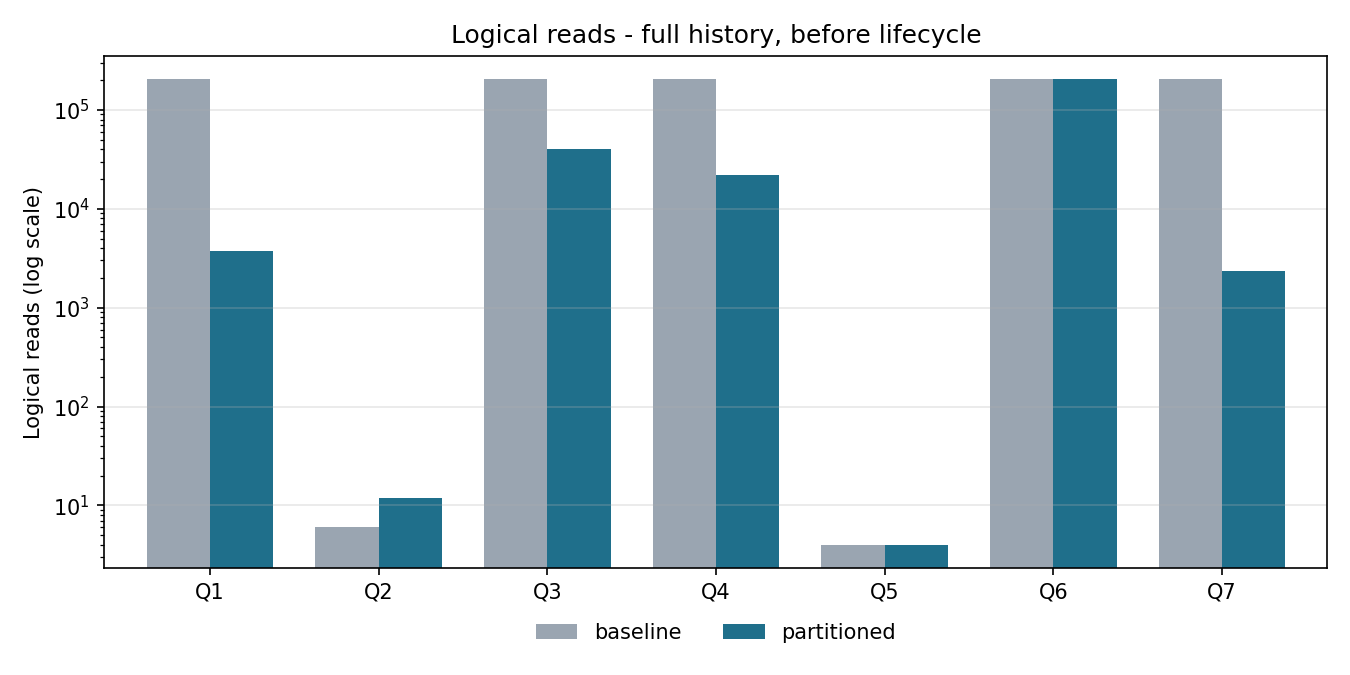
\includegraphics[width=0.92\linewidth]{queries_before_lio}
  \caption{Logical reads per query on the full history (log scale)}
  \label{fig:lio}
\end{figure}

\paragraph{Interpretation.}
\begin{itemize}
  \item \textbf{Date-bounded reports} (Q1, Q4, Q7) gain the most, because partition pruning
        reads only the requested months. The baseline full-scans the table, since a single
        month is too large a share of the rows for its \code{bill\_date} index.
  \item \textbf{Q3} reads 5--7 times fewer blocks but runs only 1.5--1.9 times faster. It
        aggregates about 4.6~million rows, so CPU dominates once I/O is gone. After the
        lifecycle, 10 of its 12 months are compressed, and decompression costs CPU.
  \item \textbf{Q6 has no date predicate}, so nothing can be pruned. Partitioning is not a
        universal accelerator. After the lifecycle Q6 reads half the blocks, because the
        online table holds 38 months, 24 of them compressed.
  \item \textbf{OLTP lookups} are unchanged in time. Q5 uses the global primary key in both
        designs. Q2 reads 12 blocks instead of 6, because the local index has one B-tree per
        month and the query covers three months. This is the cost of local indexes, and it is
        negligible here.
\end{itemize}

\begin{figure}[H]
  \centering
  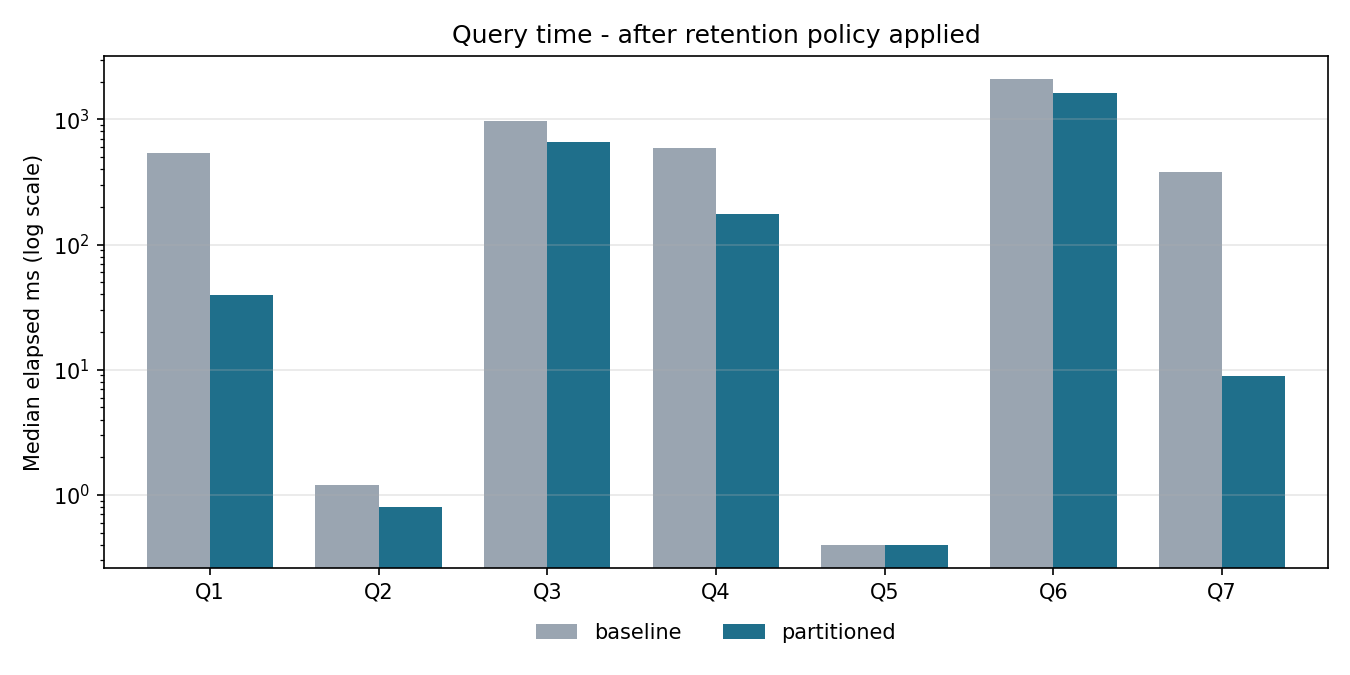
\includegraphics[width=0.92\linewidth]{queries_after_time}
  \caption{Median elapsed time per query after the retention policy (log scale)}
  \label{fig:qafter}
\end{figure}

\section{Maintenance operations}

The lifecycle was applied in steady-state order: the oldest months were warmed and archived
first, then purged \emph{from the archive}, exactly as they would be after two years in the
archive. Both designs followed this order.

\begin{table}[H]
\centering\small
\caption{Maintenance cost per operation (averages)}
\label{tab:maint}
\begin{tabularx}{\linewidth}{Lrrrrl}
\toprule
Operation (one month) & \multicolumn{2}{c}{Seconds} & \multicolumn{2}{c}{Redo (MB)} & Gain \\
& Base & Part. & Base & Part. & time \\
\midrule
Archive & 26.17 & 0.42 & 498.8 & 6.3 & 62$\times$ \\
Purge & 5.14 & 0.02 & 110.0 & $<$0.1 & $\approx$250$\times$ \\
Warm (freeze, move, compress) & -- & 3.06 & -- & 152.9 & new step \\
\textbf{Monthly job} & \textbf{31.31} & \textbf{3.51} & \textbf{608.8} & \textbf{159.3} & \textbf{8.9$\times$} \\
Load one month (429\,000 rows) & 4.36 & 2.13 & 101.9 & 76.1 & 2.0$\times$ \\
Statistics, routine refresh & 35.44 & 14.44 & 5.7 & 2.6 & 2.5$\times$ \\
Statistics, first after migration & 32.21 & 75.27 & 5.6 & 94.3 & 0.4$\times$ \\
\bottomrule
\end{tabularx}
\end{table}

The \emph{monthly job} is the fair steady-state comparison. In the baseline it is one archive
and one purge. In the partitioned design it is one warm, one archive and one purge, because
the zero-copy archive relies on the month having been compressed by the warm step. It is
8.9 times faster, with 3.8 times less redo and 4.0 times less undo. Applying the whole policy
to the six-year history at once took 1\,004~s and 19.3~GB of redo for the baseline, against
199~s and 9.4~GB for the partitioned design. Of the partitioned figures, 184~s and 9.2~GB are
the one-time warm catch-up of 60 months.

\begin{figure}[H]
  \centering
  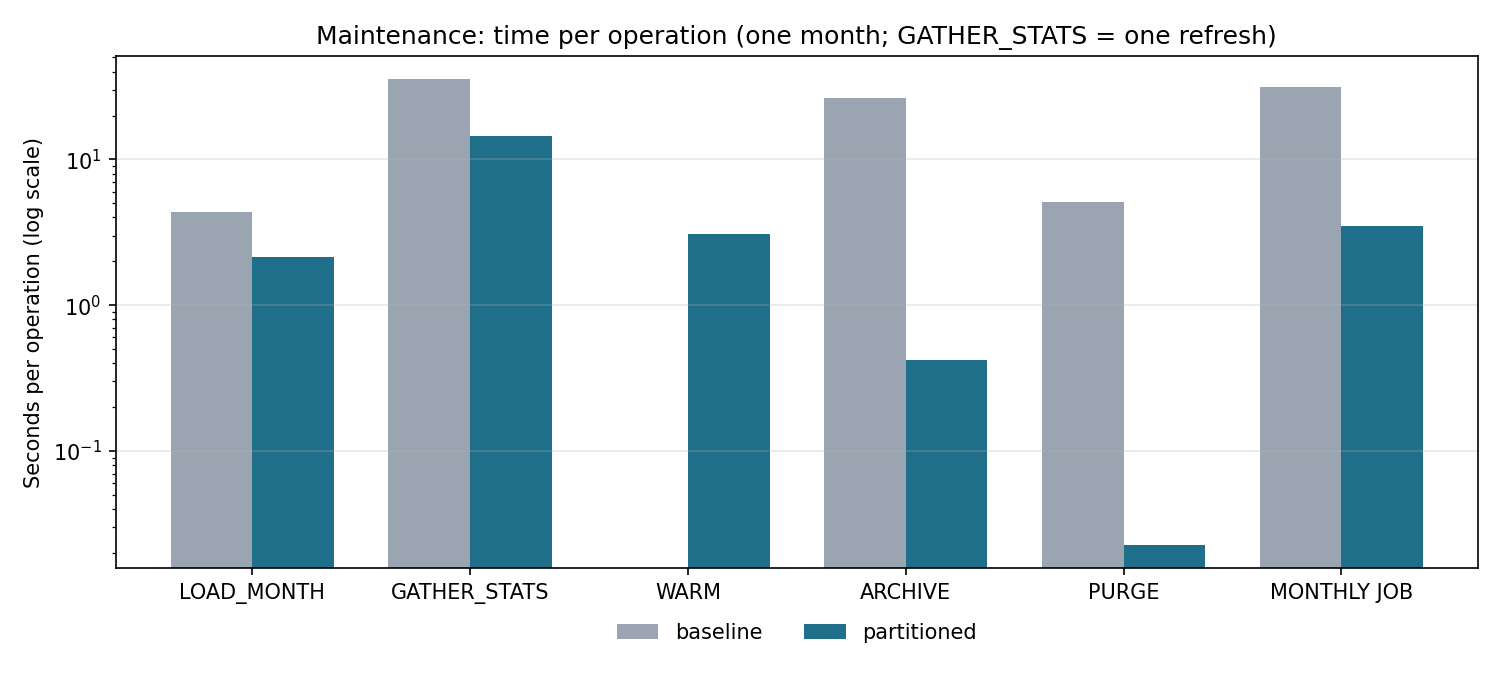
\includegraphics[width=0.95\linewidth]{maintenance_time}
  \caption{Maintenance time per operation (log scale)}
  \label{fig:maint}
\end{figure}

\paragraph{Interpretation.}
\begin{itemize}
  \item Archive and purge become metadata operations: their cost no longer depends on the
        number of rows. The baseline's \code{DELETE}s generate undo and redo for every row and
        every index entry. In ARCHIVELOG mode (production) this redo would also have to be
        archived, backed up and shipped to a standby.
  \item \textbf{WARM is the main cost of the new design} (3.1~s and 153~MB of redo per month).
        It moves and compresses the month, maintains the global primary key, rebuilds the
        local index partition and re-captures the control totals. We did not measure these
        parts separately; global index maintenance is the likely main part.
  \item The \textbf{first statistics refresh after the migration} re-analysed all 73
        partitions (75~s). The next routine refresh re-analysed only the new partition (14~s,
        2.5 times faster than the baseline). This is a one-time cost of the migration.
\end{itemize}

\section{Storage}

\begin{table}[H]
\centering
\caption{Space used, tables and their indexes (MB)}
\label{tab:space}
\begin{tabular}{lrr}
\toprule
Table & Before & After policy \\
\midrule
Baseline online (\code{BILLING\_RECORDS\_BASE}) & 3\,152 & 3\,248 \\
Baseline archive (\code{BILLING\_ARCHIVE\_BASE}, 2 indexes) & 0 & 1\,304 \\
Partitioned online (\code{BILLING\_RECORDS}) & 3\,121 & 1\,975 \\
Partitioned archive (\code{BILLING\_ARCHIVE}, 1 local index) & 0 & 587 \\
\midrule
\textbf{Retained data, baseline / partitioned} & & \textbf{4\,552 / 2\,562 (-44\,\%)} \\
\bottomrule
\end{tabular}
\end{table}

After 36 of its 74 months were moved out, the baseline table did not shrink. It even grew,
because new months were loaded above the high-water mark, and full scans still read about
212\,000 blocks. The baseline archive also keeps the space of the months deleted from it.
Releasing that space would require \code{SHRINK SPACE} or \code{MOVE} on large tables. With
partitions, a purge releases space immediately and BASIC compression shrinks warm and
archived months. The archive comparison combines compression, one index fewer and the space
the baseline did not release.

\section{Integrity and reliability}

After the whole benchmark, \textbf{62 of 62} retained months match their control totals in
both designs (row count, amount total and fingerprint sum), and every purged month is absent.
Together with the functional tests (crash and resume, interrupted warm, deliberate
corruption detected) this supports the reliability indicators K8 and K9.

\section{Indicators against targets}

\begin{longtable}{lp{0.3\linewidth}p{0.36\linewidth}l}
\caption{KPI results}\label{tab:kpiresults}\\
\toprule
KPI & Target & Result & Status \\
\midrule
\endfirsthead
\toprule
KPI & Target & Result & Status \\
\midrule
\endhead
K1 & $\geq$5$\times$ time, $\geq$10$\times$ LIO & 14$\times$ / 54--56$\times$ & met \\
K2 & $\geq$5$\times$ fewer LIO & 86$\times$ before, 97$\times$ after & met \\
K3 & no time regression $>$2$\times$ & Q5 unchanged; Q2 0.9 $\rightarrow$ 0.8~ms & met \\
K4 & archive $\geq$10$\times$, $<$5~s & archive operation 62$\times$, 0.42~s; whole monthly job 8.9$\times$, 3.5~s & met / \textbf{partly} \\
K5 & purge $<$1~s & 0.02~s & met \\
K6 & load + stats not slower & 2.0$\times$ and 2.5$\times$ faster (first gather slower, once) & met \\
K7 & $\geq$25\,\% less storage & $-$44\,\% & met \\
K8 & 100\,\% integrity & 62/62 months, both designs & met \\
K9 & 0 rows lost, re-run recovers & T12--T17, T41, Scenario 4 & met \\
K10 & 100\,\% security checks & 25/25 & met \\
K11 & one command per month & \code{dlm\_pkg.run\_lifecycle} & met \\
\bottomrule
\end{longtable}

Ten indicators are met. K4 is met for the archive operation itself (62 times faster). When
the warm step that the archive depends on is included, the whole monthly job is 8.9 times
faster, just under the 10$\times$ target. Section~\ref{sec:improvements} discusses how to
reduce the warm cost.

\chapter{Challenges Encountered and Solutions}\label{ch:challenges}

The work went through four review rounds. The last ones used independent reviewers who re-read
the code without our conclusions; every finding was checked against the code, and on the
database when Oracle's behaviour was uncertain. The main problems and their solutions follow.
The full list is in \code{docs/work\_log.md}.

\begin{longtable}{p{0.3\linewidth}p{0.3\linewidth}p{0.32\linewidth}}
\caption{Main problems and corrective actions}\label{tab:challenges}\\
\toprule
Problem & Cause / analysis & Solution \\
\midrule
\endfirsthead
\toprule
Problem & Cause / analysis & Solution \\
\midrule
\endhead
Laptop disk almost full; UNDO and TEMP could grow to 32~GB each & default autoextend of the course container & caps on every file, cleanup of unused images, free-space checks in the scripts \\
\code{sqlplus / as sysdba} failed (ORA-12162) & \code{ORACLE\_SID} not set in \code{docker exec} shells & SID passed explicitly by \code{lib.sh} \\
Partitions named \code{SYS\_Pnnn} & interval partitioning generates names & rename from \code{HIGH\_VALUE}; local index partitions matched by \emph{position} (their system names differ from the table's) \\
The application could insert a row dated in an archived month; even after \code{ROLLBACK} an empty partition remained online & interval partition creation is autonomous & application write window (view \code{WITH CHECK OPTION}); the monthly job drops empty partitions outside the window \\
Archive interrupted between the two exchanges & two DDL steps cannot be one transaction & staging table never truncated; next run detects staged rows and resumes; tested by a simulated crash \\
A bill committed between the capture of a month's totals and its move made every later run fail & order of the warm steps & freeze first (READ ONLY waits for in-flight transactions), then capture, then move (verified: MOVE is allowed on a read-only partition) \\
Read-only accounts could lock the tables and block the job & \code{SELECT} allows \code{LOCK TABLE} (verified on the DB) & \code{READ} grants; DDL waits up to 60~s for in-flight DML \\
Passwords could appear in clear text & substitution into PL/SQL literals (visible in \code{V\$SQL}); SQL*Plus echoes a failing line & users created without a password inside PL/SQL, then passwords set by plain \code{ALTER USER}; no statement can fail \\
First statistics refresh slower than the baseline (75~s) & all partitions seen as stale once after the 24~M-row migration & measured separately from the routine refresh (14~s); documented as a one-time cost \\
Purge first measured on the online table & benchmark order did not match steady state & warm and archive first, then purge from the archive, for both designs \\
Archive KPI excluded the warm step it depends on & the KPI compared one operation only & the whole monthly job is reported as well (8.9$\times$) \\
Elapsed times of baseline full scans varied widely (0.5--2.6~s for the same query) & direct-path reads always go to disk & logical reads used as the primary indicator, medians of 5 runs \\
\bottomrule
\end{longtable}

\chapter{Discussion and Future Improvements}\label{ch:discussion}

\section{Strengths}

\begin{itemize}
  \item \textbf{Measured, not claimed.} Every gain comes from the same data and workload on
        both designs, with plans, raw JSON and test outputs in the repository.
  \item \textbf{Retention as metadata.} Archive and purge no longer depend on data volume. Their
        cost stays flat as the business grows, while the baseline grows linearly.
  \item \textbf{Safety by design.} Guards refuse illegal purges, frozen data is read-only, the
        application can only write the hot window, every operation is logged and resumable,
        and integrity is proved against control totals. The job stops if a frozen month
        changes.
  \item \textbf{Operations.} One command per month, a dry-run mode, the policy stored as data,
        and readable partition names.
\end{itemize}

\section{Limitations and remaining risks}

\begin{itemize}
  \item \textbf{Licence.} Partitioning is a paid Enterprise Edition option. On Standard
        Edition~2 the design would fall back to one table per month behind a \code{UNION ALL}
        view, without basic compression (EE only) and with weaker pruning.
  \item \textbf{Queries without a date filter} gain nothing (Q6), and multi-month lookups
        through local indexes read a few more blocks (Q2).
  \item \textbf{Warm cost.} It is probably dominated by maintenance of the global primary key (not measured separately); the
        monthly job is 8.9$\times$ faster, not the 10$\times$ we targeted.
  \item \textbf{No \code{record\_id} index on archived rows}: a lookup by \code{record\_id}
        through \code{BILLING\_ALL} scans the archive partitions.
  \item \textbf{Concurrency.} The application can still hold locks (its \code{INSERT} grant
        allows \code{LOCK TABLE}), and two lifecycle runs are not serialised. Guards and row
        counts prevent data loss, but a run can fail and must be re-run.
  \item \textbf{Evaluation context.} One laptop, single-user measurements, synthetic data
        (uniform customers, no corrections of old bills) and 24~million rows. Absolute times
        are indicative; logical reads and redo are the reliable comparisons.
  \item \textbf{Owner privileges.} \code{TELCO\_OWNER} can change the policy and read
        PDB-wide \code{V\$SQL}. In production it would be locked, and the job would run under
        a scheduler with auditing on \code{DLM\_CONFIG}.
\end{itemize}

\section{Possible improvements}\label{sec:improvements}

\begin{enumerate}
  \item \textbf{Reduce the warm cost:} use \code{NOLOGGING} moves followed by a backup (only
        without a standby), warm several months in parallel off-peak, or switch to a local
        primary key on \code{(record\_id, bill\_date)} if the application can accept it.
  \item \textbf{Schedule and serialise} the monthly job with \code{DBMS\_SCHEDULER} and a
        \code{DBMS\_LOCK} lock, with alerting on \code{ERROR} or \code{REFUSED} log entries.
  \item \textbf{Archive statistics:} gather table-level synopses on \code{BILLING\_XCHG}
        before each exchange, so exchanged partitions arrive with incremental synopses.
  \item \textbf{Tiered storage:} place \code{TELCO\_ARCH} on cheaper storage and make archive
        tablespaces read-only, so backups of history are taken once.
  \item \textbf{Measure under concurrency:} run the application workload during the lifecycle
        job, and test on production-scale volumes.
  \item \textbf{Audit:} Unified Auditing policies on \code{DLM\_CONFIG} and on lifecycle
        procedures.
\end{enumerate}

\chapter{General Conclusion}\label{ch:conclusion}

The client's billing history had become a single, ever-growing table: reports were slow,
retention was an expensive \code{DELETE}, and nothing proved that billing data stayed intact.
We replaced this with a monthly partitioned design and a lifecycle package that moves each
month through four tiers: hot, warm (compressed and read-only), archive and purge. Every step
is guarded, logged, resumable and validated.

The client's objectives are met. Date-bounded reports read up to 97 times fewer blocks, and
single-month reports run 14 to 43 times faster. Archiving a month takes 0.4~s instead of 26~s,
purging one 0.02~s instead of 5~s, and the whole monthly job is 8.9 times faster with 3.8 times less redo.
Retained data uses 44\,\% less storage. All retained months match their control totals after
the whole policy. The solution passes 43 functional tests and 25 security checks, including a
crash in the middle of an archive, late inserts into old months and a deliberately corrupted
month, which the job detects and refuses to accept.

The project also showed where partitioning does not help. Queries without a date filter gain
nothing, local indexes add a few reads to multi-month lookups, and the global primary key makes
compression the main cost of the new design. These trade-offs, the licensing constraints and
the limits of a laptop evaluation are documented so the DBA Manager can decide with full
information.

Beyond the numbers, the main lesson is method. Each claim is backed by a measurement or a
test, each result can be reproduced from the repository, and each review round found real
defects that we corrected before reporting the results.

\chapter*{References}
\addcontentsline{toc}{chapter}{References}

\begin{enumerate}[label={[\arabic*]}, leftmargin=*]
  \item Oracle, \emph{Oracle Database VLDB and Partitioning Guide, 19c} -- interval
        partitioning, partition exchange, read-only partitions, partition maintenance and
        global index maintenance.
  \item Oracle, \emph{Oracle Database SQL Language Reference, 19c} -- \code{ALTER TABLE ...
        MOVE / EXCHANGE / DROP PARTITION}, \code{LOCK TABLE}, \code{CREATE VIEW ... WITH CHECK
        OPTION}, \code{READ} object privilege.
  \item Oracle, \emph{Oracle Database SQL Tuning Guide, 19c} -- incremental statistics,
        partition pruning, \code{DBMS\_XPLAN}.
  \item Oracle, \emph{Oracle Database PL/SQL Packages and Types Reference, 19c} --
        \code{DBMS\_STATS}, \code{DBMS\_XPLAN}, \code{DBMS\_UTILITY}, \code{DBMS\_ASSERT}.
  \item Oracle, \emph{Oracle Database Licensing Information User Manual, 19c} -- Partitioning,
        Advanced Compression, Diagnostics and Tuning Packs, basic table compression.
  \item Oracle, \emph{Oracle Database Reference, 19c} -- \code{V\$MYSTAT}, \code{V\$STATNAME},
        \code{V\$SESSION}, \code{V\$SQL}, \code{USER\_TAB\_PARTITIONS}.
  \item Oracle, \emph{docker-images} repository, \code{OracleDatabase/SingleInstance} build
        files (\url{https://github.com/oracle/docker-images}).
  \item \emph{python-oracledb documentation}, Oracle (\url{https://python-oracledb.readthedocs.io}).
  \item Course material: \emph{General Project Guidelines} and \emph{Project 22} specification
        (\code{docs/assignment/}).
\end{enumerate}

\paragraph{Use of AI tools.} An AI assistant (Claude) was used to help design and write
scripts and documentation and to run code reviews. All code was executed and validated by the
automated tests and the benchmark in the repository, and the team is responsible for the
content of this report.


\appendix
\chapter{Team Organisation and Schedule}

\section{Four-week plan}

\begin{table}[H]
\centering
\caption{Project schedule}
\begin{tabularx}{\linewidth}{lLL}
\toprule
Week & Activities & Outcome \\
\midrule
1 & Requirements, environment assessment, technology comparison, architecture, indicators & validated design, prepared environment (tablespace caps, accounts) \\
2 & Schema, data generator, partitioned design, lifecycle and baseline packages & first working version \\
3 & Functional and security tests, incident simulation, benchmark, review rounds and corrections & verifiable results \\
4 & Final benchmark, demonstration rehearsal, report and presentation & final solution and defense \\
\bottomrule
\end{tabularx}
\end{table}

\section{Distribution of responsibilities}

Both members can explain the whole solution. Each area has an owner, who presents it and
answers first, and a reviewer.

\begin{table}[H]
\centering
\caption{Responsibilities}
\begin{tabularx}{\linewidth}{Lll}
\toprule
Area & Owner & Reviewer \\
\midrule
Requirements, client scenario, indicators, technology assessment & \TeamMemberA & \TeamMemberB \\
Architecture, partitioning and indexing design & \TeamMemberA & \TeamMemberB \\
Lifecycle package (\code{DLM\_PKG}) & \TeamMemberA & \TeamMemberB \\
Environment, tablespaces, accounts, security & \TeamMemberB & \TeamMemberA \\
Data generator, baseline design, data loading & \TeamMemberB & \TeamMemberA \\
Functional, security and incident tests & \TeamMemberB & \TeamMemberA \\
Benchmark harness and result analysis & \TeamMemberA & \TeamMemberB \\
Demonstration, report and presentation & both & -- \\
\bottomrule
\end{tabularx}
\end{table}

\chapter{Lifecycle Package Interface}

\needspace{0.3\textheight}
\begin{lstlisting}[style=sql, caption={Specification of \code{DLM\_PKG} (abridged)}]
create or replace package dlm_pkg authid definer as
  function  get_param(p_name in varchar2) return varchar2;
  function  as_of_month return date;
  procedure log_event(p_run_id, p_job, p_action, p_target, p_rows, p_elapsed,
                      p_status, p_message default null);      -- autonomous
  function  partition_month(p_table in varchar2, p_partition in varchar2) return date;
  function  partition_for(p_table in varchar2, p_month in date) return varchar2;
  procedure rename_partitions(p_table in varchar2);
  procedure warm_partition   (p_month in date, p_run_id in number default null,
                              p_as_of in date default null);
  procedure archive_partition(p_month in date, p_run_id in number default null,
                              p_simulate_failure in varchar2 default null,
                              p_as_of in date default null);
  procedure purge_partition  (p_month in date, p_run_id in number default null,
                              p_retention_months in pls_integer default null,
                              p_as_of in date default null);
  procedure refresh_app_window(p_as_of in date default null);
  procedure run_lifecycle(p_as_of in date default null, p_dry_run in boolean default false);
  procedure capture_control_totals(p_table in varchar2);
  procedure capture_month_totals(p_table in varchar2, p_month in date);
  function  validate_integrity(p_view in varchar2, p_from_month in date default null,
                               p_run_id in number default null,
                               p_to_month in date default null) return number;
end dlm_pkg;
\end{lstlisting}

\begin{table}[H]
\centering
\caption{Error codes raised by the lifecycle code}
\begin{tabularx}{\linewidth}{lL}
\toprule
Code & Meaning \\
\midrule
ORA-20010 & operation refused by a guard (retention, online or hot window, foreign staged month) \\
ORA-20020 & simulated failure (tests and demonstration only) \\
ORA-20030 & row count mismatch after an archive \\
ORA-20040 & integrity validation failed at the end of a monthly run \\
ORA-20050 & another lifecycle operation is already running (job lock) \\
ORA-20098 & functional tests refused (wrong calendar, dataset not fresh or too large) \\
ORA-20099 & one or more automated tests failed \\
\bottomrule
\end{tabularx}
\end{table}

\chapter{Test Output (excerpt)}

\needspace{0.3\textheight}
\begin{lstlisting}[style=console, caption={\code{results/tests/functional\_tests.txt} (excerpt)}]
PASS  T01 partitioned copy matches control totals
PASS  T03 dry run plans 12 purges
PASS  T07 purge refused when retention < legal floor (24 < 60)  (got ORA-20010 ...)
PASS  T37 purge refused at the retention boundary (2021-11)  (got ORA-20010 ...)
PASS  T12 simulated crash after exchange step 1  (got ORA-20020 ...)
PASS  T13 no row lost during the crash: rows wait in BILLING_XCHG  (2404 rows staged)
PASS  T15 re-run resumes and completes the archive
PASS  T34 warm of a system-named partition rebuilds its local index (by position)
PASS  T35 re-running an interrupted warm completes it (index rebuilt, read only)
PASS  T42 every archive partition is compressed, read-only, in TELCO_ARCH
PASS  T25 second run is a no-op (idempotent: no operation performed)
PASS  T26 archived data cannot be modified (read-only partition)  (got ORA-14466 ...)
PASS  T32 lifecycle succeeds after the application committed new HOT rows
PASS  T41 run_lifecycle resumes the crashed archive (step 0a)
PASS  T40 lifecycle stops (ORA-20040) when a frozen month was altered
PASS  T33 baseline lifecycle archives 24 months and keeps every retained row
----------------------------------------------
Tests passed: 43   failed: 0
\end{lstlisting}

\chapter{Reproducing the Results}

\begin{lstlisting}[style=bash]
git clone https://github.com/Baounna/oracle-billing-lifecycle.git && cd oracle-billing-lifecycle
scripts/init_env.sh
scripts/01_setup_db.sh && scripts/02_create_schema.sh && scripts/03_load_data.sh
scripts/05_benchmark.sh              # results/summary.md, results/charts/
# functional and security tests on the smoke dataset:
(umask 077; sed -e 's/^ROWS_PER_MONTH=.*/ROWS_PER_MONTH=3000/' \
                -e 's/^CUSTOMERS=.*/CUSTOMERS=5000/' .env > .env.smoke)
( export ENV_FILE=$PWD/.env.smoke; scripts/reset.sh --yes && scripts/01_setup_db.sh \
  && scripts/02_create_schema.sh && scripts/03_load_data.sh && scripts/04_run_tests.sh )
\end{lstlisting}


\end{document}
